\documentclass{scrartcl}

\emergencystretch2em

\usepackage[utf8]{inputenc}
\usepackage[T1]{fontenc}
\usepackage[ngerman]{babel}
\usepackage{verbatim}
\usepackage[widespace]{fourier}
\usepackage{geometry,mathtools,amsmath}
\usepackage{tikz}
\usetikzlibrary{arrows.meta}
\usetikzlibrary{petri,topaths,matrix,chains,positioning,decorations.pathreplacing,arrows}
\usetikzlibrary{calc,decorations.pathmorphing,patterns}
\usetikzlibrary{calc} % 2, 3, 4
\usetikzlibrary{decorations.shapes,shapes} % 3
\usetikzlibrary{patterns}
\usepackage{tkz-graph}
\usepackage{tkz-berge}
\usepackage{qtree}
\usepackage{soulutf8}
\usepackage[shortlabels]{enumitem}
\usepackage{color, colortbl}
\definecolor{LightCyan}{rgb}{0.56,0.93,0.56}
\definecolor{HeavyRed}{rgb}{1,0,0}
\usetikzlibrary{tikzmark}
\usepackage{array}
\usepackage{mathtools}
\usepackage{xcolor,cancel}
\usetikzlibrary{trees}
\usepackage[pdf]{graphviz}
\usepackage{caption}
\usepackage{subcaption}
\usepackage{wrapfig}

\newcommand*{\QEDA}{\hfill\ensuremath{\blacksquare}}%
\newcommand*{\QEDB}{\hfill\ensuremath{\square}}%

\newcommand{\ro}[1]{\ensuremath{\overline{\textrm{\underline{#1}}}}}
\newcommand{\ggt}[1]{\ensuremath{\textrm{ggT}\left(#1\right)}}
\usepackage{amssymb}% http://ctan.org/pkg/amssymb
\usepackage{pifont}% http://ctan.org/pkg/pifont
\def\checkmark{\tikz\fill[scale=0.4](0,.35) -- (.25,0) -- (1,.7) -- (.25,.15) -- cycle;}
\newcommand{\cmark}{\textcolor{green}{\checkmark}}
\newcommand{\mystar}{{\textcolor{red}{\fontfamily{lmr}\selectfont\ensuremath{\star}}}}
\newcommand{\xmark}{\textcolor{red}{X}}
\newcommand{\importantmark}{\textcolor{red}{\danger}\ }
\newcommand\hcancel[2][black]{\setbox0=\hbox{$#2$}%
\rlap{\raisebox{.45\ht0}{\textcolor{#1}{\rule{\wd0}{1pt}}}}#2} 

\usepackage{nameref}

\newcommand{\TODO}{{\Huge\textcolor{HeavyRed}{\danger !!!TODO!!! \danger}}}

\newcommand{\picturetext}[2]{%
\begin{minipage}{.45\linewidth}%
#1%
\end{minipage}\hfill%
\begin{minipage}{.45\linewidth}%
#2%
\end{minipage}%
\vspace{3em}%
}

\usepackage{pgfplots}
\pgfplotsset{compat=newest}

\usetikzlibrary{automata}
\usetikzlibrary{graphs}

\usetikzlibrary{calc,trees,positioning,arrows,chains,shapes.geometric,%
    shapes,shadows,matrix}
\usepackage{tikzpeople}

\newcommand{\stargraph}[2]{\begin{tikzpicture}
    \node[circle,fill=black] at (360:0mm) (center) {$0$};
    \foreach \n in {1,...,#1}{
        \node[circle,fill=black] at ({\n*360/#1}:#2cm) (n\n) {$\n$};
        \draw (center)--(n\n);
        \node at (0,-#2*1.5) {$S_{#1}$}; % delete line to remove label
    }
\end{tikzpicture}}


\usepackage[
	hidelinks,
	breaklinks=true,
	pdftex,
	pdfauthor={Norman Koch, Lukas Malte Causse},
	pdfsubject={},
	pdfkeywords={},
	pdfproducer={},
	pdfcreator={}]{hyperref}

\author{Norman Koch, Lukas Malte Causse}
\title{Lernhilfe LA1/DIS1}

\newcommand{\ExternalLink}{%
    \tikz[x=1.2ex, y=1.2ex, baseline=-0.05ex]{% 
        \begin{scope}[x=1ex, y=1ex]
            \clip (-0.1,-0.1) 
                --++ (-0, 1.2) 
                --++ (0.6, 0) 
                --++ (0, -0.6) 
                --++ (0.6, 0) 
                --++ (0, -1);
            \path[draw, 
                line width = 0.5, 
                rounded corners=0.5] 
                (0,0) rectangle (1,1);
        \end{scope}
        \path[draw, line width = 0.5] (0.5, 0.5) 
            -- (1, 1);
        \path[draw, line width = 0.5] (0.6, 1) 
            -- (1, 1) -- (1, 0.6);
        }
}

\newcommand*{\fullref}[1]{\hyperref[{#1}]{\hbox{\ExternalLink\textit{\nameref*{#1}} (\ref{#1})}}}

\usepackage{titlesec}
\newcommand{\sectionbreak}{\clearpage}
\usepackage{url}

%\RedeclareSectionCommand[tocnumwidth=2.6em]{section}
%\RedeclareSectionCommand[tocindent=4.1em,tocnumwidth=3.5em]{subsection}
\RedeclareSectionCommand[tocnumwidth=4em]{subsubsection}

\begin{document}

\maketitle

\newpage

\tableofcontents

\newpage

\section{Vorwort}

Dieses Dokument stellt nach bestem Wissen und Gewissen mein Verständnis des im ersten Semester der Informatik an der TU Dresden
in Linearer Algebra und Diskreten Strukturen dar. Ich erhebe weder Anspruch auf Vollständigkeit noch auf Richtigkeit meines
Verständnisses noch der hier behandelten Themen.

Ich stelle dieses Dokument unter die WTFPL\footnote{Siehe dazu \url{http://www.wtfpl.net/}.}. Jeder kann damit machen, was er oder sie möchte, und das völlig ohne Einschränkungen
jedweder Art. Gleichzeitig bin ich aber für das, was Jemand mit diesem Dokument macht, nicht verantwortlich.

\newpage

\section{Allgemeine Tipps}

\subsection{Herleitung der Potenzgesetze}

Das habe ich mir im Abi überlegt und das einmal gerafft zu haben (und nicht blind dogmatisch einfach angenommen zu haben)
hat mir bisher immer ganz gut geholfen.

\subsubsection{Warum ist $x^0 = 1$? Warum ist $x^{-1} = \frac{1}{x}$?}

$$
\dots
$$

\begin{equation}
x \times x \times x = x^3 \tag*{: x}
\end{equation}

\begin{equation}
\frac{x \times x \times x}{x} = x \times x = x^2 \tag*{: x}
\end{equation}

\begin{equation}
\frac{x \times x \times x}{x \times x} = x = x^1 \tag*{: x}
\end{equation}

\begin{equation}
\frac{x \times x \times x}{x \times x \times x} = 1 = x^0 \tag*{: x}
\end{equation}

\begin{center}
	\danger: Wenn $x = 0$, dann hätte man $\frac{0}{0}$, daher $0^0 = $ undef.
\end{center}

\begin{equation}
\frac{x \times x \times x}{x \times x \times x \times x} = \frac{\hcancel[red]{x \times x \times x} \rightarrow 1}{\hcancel[red]{x \times x \times x \times} \rightarrow 1 x} = \frac{1}{x} = x^{-1} \tag*{: x}
\end{equation}

\begin{equation}
\frac{x \times x \times x}{x \times x \times x \times x} = \frac{\hcancel[red]{x \times x \times x} \rightarrow 1}{\hcancel[red]{x \times x \times x \times} \rightarrow 1 x \times x} = \frac{1}{x \times x} = x^{-2} \tag*{: x}
\end{equation}

$$
\dots
$$


\subsubsection{Warum ist $x^n \cdot x^m = x^{n + m}$?}

Nehmen wir das Beispiel
\begin{equation}
	x^3 \cdot x^5,
\end{equation}
das bedeutet,
\begin{equation}
	(x \cdot x \cdot x) \cdot (x\cdot x\cdot x\cdot x\cdot x),
\end{equation}
was wegen der Assoziativität bedeutet:
\begin{equation}
	x \cdot x \cdot x \cdot x\cdot x\cdot x\cdot x\cdot x,
\end{equation}
was das Gleiche ist wie
\begin{equation}
	x^{3 + 5} = x^8.
\end{equation}

Ich kann es nicht beweisen, aber es ist (für mich zumindest) ersichtlich, dass diese Regel aufgrund der Assoziativität
der Multiplikation allgemeingültig ist.

Gleiches gilt übrigens für alle $x^r, r\in\mathbb{R}$, denn z.\,B.
\begin{equation}
	x^3 \cdot x^{-2} = (x \cdot x \cdot x) \cdot (\frac{1}{x\cdot x}) = 
	\frac{\hcancel[red]{x\cdot x}\rightarrow 1\cdot x}{\hcancel[red]{x\cdot x}\rightarrow 1} =
	\frac{x}{1} = x^1 = x^{3 - 2}.
\end{equation}

\subsubsection{Warum ist $\left(x^n\right)^m = \left(x^m\right)^n = x^{n\cdot m}$?}

\label{warumxhochn}

Nehmen wir auch hier ein konkretes Beispiel:

\begin{equation}
	\left(2^3\right)^2 = \left(2\cdot 2 \cdot 2\right)^2 = \left(2\cdot 2 \cdot 2\right) \cdot \left(2\cdot 2 \cdot 2\right) = 
	2\cdot 2 \cdot 2 \cdot 2\cdot 2 \cdot 2 = 2^6 = 2^{2\cdot 3}.
\end{equation}

Vertauschen wir $m$ und $n$, dann erhalten wir:

\begin{equation}
	\left(2^2\right)^3 = \left(2\cdot 2\right)^3 = \left(2\cdot 2\right) \cdot \left(2\cdot 2\right) \cdot \left(2\cdot 2\right) =
	2\cdot 2 \cdot 2 \cdot 2\cdot 2 \cdot 2 = 2^6 = 2^{3\cdot 2}.
\end{equation}

Auch hier kann ich es nicht allgemein \textit{beweisen}, halte es aber, wenn man es im konkreten Fall sieht,
für einleuchtend auch im Allgemeinen Fall.

\subsubsection{Warum ist $x^{\frac{1}{n}} = \sqrt[n]{x}$?}

Dadurch, dass $x^n \times x^m = x^{n + m}$ ist, können wir einsehen, dass

\begin{equation}
	x^\frac{1}{n} \cdot x^\frac{1}{n} = x^{\frac{1}{n} + \frac{1}{n}} = x^\frac{2}{n}.
\end{equation}

Daraus folgt im spezifischen Fall z.\,B. für $n = 2$:

\begin{equation}
	x^\frac{1}{2} \cdot x^\frac{1}{2} = x^\frac{2}{2} = x^1.
\end{equation}

Die Zahl, die mit sich selbst multipliziert $n$ ergibt, nennen wir auch $\sqrt{n}$. Daher gilt:

\begin{equation}
	x^\frac{1}{2} = \sqrt{n}.
\end{equation}

Gleiches gilt z.\,b. für $x^\frac{1}{3}$, denn:

\begin{equation}
	x^\frac{1}{3} \cdot x^\frac{1}{3} \cdot x^\frac{1}{3} = x^{\frac{1}{3} + \frac{1}{3} + \frac{1}{3}} = x^\frac{3}{3} = x^1,
\end{equation}
weshalb $x^\frac{1}{3} = \sqrt[3]{x}$ ist und allgemein $x^\frac{1}{n} = \sqrt[n]{x}$.

\subsubsection{Warum ist $x^\frac{a}{n} = \sqrt[n]{x^a}$?}

Nehmen wir wieder ein konkretes Beispiel.

\begin{equation}
	2^\frac{3}{2} \cdot 2^\frac{3}{2} = 2^{\frac{3}{2} + \frac{3}{2}} = \left(2^{\frac{1}{2}}\right)^3.
\end{equation}

Aufgrund der Assoziativität der Multiplikation kann man hier die innere und die äußere Potenz beliebig tauschen.
Wir erhalten:

\begin{equation}
	\left(2^3\right)^\frac{1}{2} = \sqrt[2]{2^3}.
\end{equation}


Ersetzt man die konkreten Zahlen durch Variablen und erhöhlt dementsprechend die
Anzahl der Multiplikationen, ist deutlich, dass dies allgemein gilt.

\subsection{Komplizierte Binominale relativ schnell ausrechnen}

Um etwas wie $(a + b)^6$ schnell auszurechnen, nehmen wir das pascal'sche Dreieck bis zur sechsten Zeile:

\begin{equation}
\begin{tabular}{>{$n=}l<{$\hspace{12pt}}*{13}{c}}
0 &&&&&&&1&&&&&&\\
1 &&&&&&1&&1&&&&&\\
2 &&&&&1&&2&&1&&&&\\
3 &&&&1&&3&&3&&1&&&\\
4 &&&1&&4&&6&&4&&1&&\\
5 &&1&&5&&10&&10&&5&&1&\\
6 &1&&6&&15&&20&&15&&6&&1
\end{tabular}
\end{equation}


Dazu nehmen wir die 6. Zeile als Vorfaktor und lassen von links nach rechts für je $a$ die Potenzen von 6 bis
0 laufen und für $b$ von 0 bis 6. Wir erhalten:

\begin{equation}
	%1	6	15	20	15	6	1
	a^6\cdot b^0 + 6a^5\cdot b^1 + 15a^4\cdot b^2 + 20a^3\cdot b^3 + 15a^2\cdot b^4 + 6a^1\cdot b^5 + a^0\cdot b^6 =
\end{equation}
\begin{equation*}
	a^6 + 6a^5\cdot b + 15a^4\cdot b^2 + 20a^3\cdot b^3 + 15a^2\cdot b^4 + 6a\cdot b^5 + b^6
\end{equation*}

Das pascal'sche Dreieck bietet übrigens auch \frq Shortcuts\flq\ zu einigen Binominalkoeffizienten, nämlich so:

\begin{center}
\begin{equation}
\begin{tikzpicture}
	\foreach \n in {0,...,4} {
		\foreach \k in {0,...,\n} {
			\node at (\k-\n/2,-\n) {$\binom{\n}{\k}$};
		}
	}
\end{tikzpicture}
\end{equation}
\end{center}

\section{Gesetze der Logik und Algebra}

\subsection{Transitivität}

\begin{equation}
	x = y \wedge y = z \implies x = z,
\end{equation}
\begin{equation}
	x < y \wedge y < z \implies x < z.
\end{equation}

\subsection{Kommutativgesetz}

\begin{equation}
	a \circ b = b \circ a
\end{equation}

\subsection{Assoziativgesetz}

\begin{equation}
	(a \circ b) \circ c = b (\circ a \circ c)
\end{equation}


\subsection{Distributivgesetz}

\begin{equation}
	a \cdot (b \diamond c) = (a \cdot b) \diamond (a \cdot c)
\end{equation}


\section{Diskrete Strukturen}

\subsection{Logische Prinizpien}

\subsubsection{Darstellungssatz}

Der Darstellungssatz besagt, % vielleicht
dass jede einvariablige logische Präposition dargestellt werden kann als

\begin{equation}
	\bigvee\bigwedge l,
\end{equation}
wobei $l$ ein Literal ist, d.\,h. entweder $\lnot x$ oder $x$.

\subsubsection{Äquivalenzen}

Es gilt das sogenannte Zirkelschlussprinzip. Das besagt:

\begin{equation}
	\left(\left(x_1 \Rightarrow x_2\right) \wedge \left(x_2 \Rightarrow x_3\right) \wedge \left(x_3 \Rightarrow x_4\right) \wedge \left(x_4 \Rightarrow x_1\right)\right) \equiv \bigwedge_{i \in \{1, \dots, n\}} \left(x_i \Leftrightarrow x_1 \right)
\end{equation}

Das heißt, dass von jedem Schluss auf jeden anderen (logisch) geschlossen werden kann.

\subsection{Die Russellsche Antinomie}

Sagen wir, wir definieren die Menge aller Mengen, die sich nicht selbst beinhalten:

\begin{equation}
	M = \{x | x \not\in x\}
\end{equation}

Dann erhalten wir ein Paradox: beinhaltet die Menge sich selbst, dann darf sie sich nicht
selbst beinhalten und darf nicht in die Liste (muss aber dafür vorher in der Liste gewesen sein).
Beinhaltet sie sich nicht selbst, dann muss sie in Liste und darf dementsprechend wieder nicht in
der Liste sein.

Dieses Problem lösen wir rein praktisch durch eine minimale Form der Typentheorie, nämlich so,
dass man die Eingabemenge beschränkt. Mit:

\begin{equation}
	M = \{x \in \mathbb{N} | x \not\in x\}
\end{equation}
entsteht dieses Paradox nicht, da in $\mathbb{N}$ keine Mengen sind, sondern konkrete einzelne
Objekte.

\subsection{Gödels Unvollständigkeitssätze}

Gödels Unvollständigkeitssätze besagen, dass jedes formale System, aus dem Etwas wie natürliche Zahlen
und die Multiplikation heraus definierbar sind, entweder

\begin{itemize}
	\item Sätze beinhalten, die nicht bewiesen werden können, aber wahr sind, oder, wenn das System beweisen kann,
		dass es vollständig ist,
	\item dass das System dann notwendigerweise widersprüchlich sein muss.
\end{itemize}

Das heißt, man kann nie per Algorithmus alle wahren Aussagen aus einem ausreichend-komplexen formalen
System auch beweisen.

Eine (sehr vereinfachte) Weise, sich solche Sätze vorzustellen, wäre z.\,B. \frq dieser Satz ist nicht beweisbar\flq.
Wäre er beweisbar, wäre er wahr, also wäre er nicht beweisbar.

\subsection{Die Potenzmenge}

Die Potenzmenge einer Menge wird bezeichnet mit $\mathcal{P}(A)$ und beschreibt die Menge aller aus der Menge
$A$ bildbaren Untermengen.

Die Potenzmenge der leeren Menge ist die Menge mit dem Element der leeren Menge: $\mathcal{P}(\emptyset) = \{\emptyset\}$.

Die Kardinalität der Potenzmenge bei endlichen Mengen ist $|\mathcal{P}(A)| = 2^{|A|}$. Die Potenzmengen unendlicher
Mengen sind strikt größer als die Ursprungsmengen.

\subsection{Binominalkoeffizienten}

Der Binominalkoeffizient gibt an, wie viele Möglichkeiten es gibt, aus $n$ Elementen $k$ auszuwählen, z.\,B. wie
viele Möglichkeiten es gibt, beim Lotto $k = 6$ Zahlen aus $n = 49$ auszuwählen.

Das schreibt man so:

\begin{equation}
	\binom{n}{k} = \binom{49}{6}.
\end{equation}

Die konkrete Zahl bestimmt sich aus

\begin{equation}
	\binom{n}{k} = \frac{n!}{k!\cdot(n - k)!}.
\end{equation}

Konkret für das Beispiel der Lottoziehung heißt das:

\begin{equation}
	\binom{49}{6} = 
	\frac{49!}{6!\cdot(49 - 6)!} =
	\frac{49!}{6!\cdot43!} =
\end{equation}
\begin{equation*}
	\frac{49 \cdot 48 \cdot 47 \cdot 46 \cdot 45 \cdot  44 \cdot  \hcancel[red]{43!}}{(6 \cdot 5 \cdot 4 \cdot 3 \cdot 2) \cdot \hcancel[red]{43!}} =
\end{equation*}
\begin{equation*}
	\frac{49 \cdot 48 \cdot 47 \cdot 46 \cdot 45 \cdot  44}{6 \cdot 5 \cdot 4 \cdot 3 \cdot 2} = \frac{10068347520}{720} = 13983816
\end{equation*}

Das heißt, dass die Wahrscheinlichkeit, die richtigen 6 Zahlen zu ziehen, $1 : 13983816$ ist (also etwa $0,00000715\%$).

Für ein einfacheres Beispiel, sagen wir, wir haben 5 Murmeln und ziehen daraus 3 heraus, heißt das, es gibt

\begin{equation}
	\binom{5}{3} =
	\frac{5!}{3!\cdot(5 - 3)!} =
	\frac{5!}{3!\cdot 2!} =
	\frac{5\cdot 4 \cdot 3 \cdot 2}{3\cdot 2 \cdot 2} =
	\frac{120}{12} = 10
\end{equation}
$\rightarrow$ 10 Kombination von Dreiermurmeln, wie wir aus den 5 Murmeln rausziehen können\footnote{Das lässt sich auch ausdrücken
als $|M| = 5, \left|\left\{ N \middle| N\in \mathcal{P}(M) \wedge |N| = 3 \right\}\right| = 10$.}.

\subsection{Permutationen}

Eine Permutation ist eine bijektive Funktion, die $A$ nach $B$ eineindeutig abbildet.

Hat man z.\,B. die ersten drei natürlichen Zahlen und permutiert sie z.\,B. so, dass jede Zahl \frq nach rechts
verschoben\flq\ wird, dann ergibt sich folgende Permutation:

\begin{equation}
	P_1 = \begin{pmatrix*}
		1 & 2 & 3\\
		3 & 1 & 2\\
	\end{pmatrix*}.
\end{equation}

1 bildet hier auf 3 ab, 2 auf 1 und 3 auf 2. 

Komponiert man Permutationen, fängt man im hintersten Element an und arbeitet sich dann Wert für Wert nach vorne.
Das Komponieren von Permutationen ist \textbf{nicht} assoziativ, d.\,h. im allgemeinen Fall $p_1 \circ p_2 \not= p_2 \circ p_1$.

\begin{equation}
	P_1 = \begin{pmatrix*}
		1 & 2 & 3\\
		3 & 1 & 2\\
	\end{pmatrix*}, 
	P_2 = \begin{pmatrix*}
		1 & 2 & 3\\
		3 & 1 & 2\\
	\end{pmatrix*}
\end{equation}

\begin{equation}
	P_1 \circ P_2 = \begin{pmatrix*}
		1 & 2 & 3 \\
		2 & 3 & 1\\
	\end{pmatrix*}
\end{equation}

Solange die Ordnung bewahrt bleibt, ist die Reihenfolge, in der die Werte aufgeschrieben werden,
egal (das heißt: man muss quasi das Bild \frq rotieren\flq\ können, als wäre es auf einem dreidimensionalen
Zylinder angeordnet).

\subsection{Boole'sche Funktionen}

Boole'sche Funktionen haben als Eingabemenge $B^n = \{0, 1\}^n$ und als Ausgabemenge die Menge
$B = \{0, 1\}$. Wir können diese Werte verstehen als \frq $0 = $ False\flq\ und \frq $1 = $ True\flq.

\subsection{Das DeMorgan'sche Gesetz}

\label{DeMorgan}

Kurz gesagt: $\lnot(x \wedge y) = \lnot x \lor \lnot y$. Wenn nötig, Beweis durch Wahrheitstabelle.

\subsection{Erfüllbarkeit}

Eine Aussage $P$ ist dann erfüllbar, wenn es eine Variablenbelegung gibt, für die $P$ ein wahrer Ausdruck ist.

Beispiel:

\begin{equation}
	P = (X \wedge Y) \lor (X \wedge \lnot Y)
\end{equation}

$P$ ist dann erfüllt, wenn $X$ wahr ist. Der Wahrheitswert von $Y$ spielt hier keine Rolle. $P$ ist also erfüllbar, weil
es eine Belegung gibt, für die $P$ ein wahrer Satz ist.

\subsection{Konjunktive/Disjunktive Normalform}

\label{knfdnf}

Die konjunktive/disjunktive Normalform sieht beispielsweise folgendermaßen aus:

\paragraph{Konjunktive Normalform:} $(A \lor B \lor \lnot C) \wedge (D \lor E \lnot F)$. Die Struktur ist, dass wir mindestens eine
Klausel haben, die in der Klausel mit dem $\bigvee$ verbunden ist und die Klauseln als Ganzes sind mit dem $\bigwedge$ verbunden.

\paragraph{Disjunktive Normalform:} $(A \wedge B \wedge \lnot C) \lor (D \lor E \lnot F)$. Die Struktur ist, dass wir mindestens eine
Klausel haben, die in der Klausel mit dem $\bigwedge$ verbunden ist und die Klauseln als Ganzes sind mit dem $\bigvee$ verbunden.

Wir erhalten aus einer Wahrheitstabelle die KNF, in dem wir uns nur die falschen Werte ansehen und dann entsprechend negieren.
Beispiel:

\begin{table}[h!]
\begin{tabular}{l|l|l|l|l|}
\cline{2-5}
Nummer & $A$ & $B$ & $C$ & $F$ \\ \cline{2-5}
1      & 0 & 0 & 0 & 1 \\ \cline{2-5}
2      & 0 & 0 & 1 & 1 \\ \cline{2-5}
3      & 0 & 1 & 0 & 1 \\ \cline{2-5}
4      & 0 & 1 & 1 & 1 \\ \cline{2-5}
5      & 1 & 0 & 0 & 0 \\ \cline{2-5}
6      & 1 & 0 & 1 & 1 \\ \cline{2-5}
7      & 1 & 1 & 0 & 0 \\ \cline{2-5}
8      & 1 & 1 & 1 & 1 \\ \cline{2-5}
\end{tabular}
\end{table}

Interessant sind hier die Zeilen mit der Nummer 5 und 7, denn diese sind 0. Um sie aus den Werten $A$, $B$ und $C$ zu generieren,
müssen wir folgende Formeln annehmen:

\begin{equation}
	P = (\lnot A \lor B \lor C) \wedge (\lnot A \lor \lnot B \lor C)
\end{equation}
und haben somit die KNF gefunden.

Bei der DNF schauen wir uns nur die wahren Zeilen an:

\begin{table}[h!]
\begin{tabular}{l|l|l|l|l|}
\cline{2-5}
Nummer & $A$ & $B$ & $C$ & $F$ \\ \cline{2-5}
1      & 0 & 0 & 0 & 0 \\ \cline{2-5}
2      & 0 & 0 & 1 & 0 \\ \cline{2-5}
3      & 0 & 1 & 0 & 0 \\ \cline{2-5}
4      & 0 & 1 & 1 & 0 \\ \cline{2-5}
5      & 1 & 0 & 0 & 1 \\ \cline{2-5}
6      & 1 & 0 & 1 & 0 \\ \cline{2-5}
7      & 1 & 1 & 0 & 1 \\ \cline{2-5}
8      & 1 & 1 & 1 & 0 \\ \cline{2-5}
\end{tabular}
\end{table}

(Wieder 5 und 7, nur diesmal exakt andersherum)

Wir schauen uns an, welche Werte negiert werden müssen, um in der Disjunktion zu diesen Falschheitswerten zu kommen und
wenden das DeMorgan'sche Gesetz (vgl. \fullref{DeMorgan}) an.

\begin{equation}
	P = \lnot(\lnot A \wedge B \wedge C) \lor \lnot(\lnot A \wedge \lnot B \wedge C) =
\end{equation}
\begin{equation*}
 (A \wedge \lnot B \wedge \lnot C) \lor (A \wedge B \wedge \lnot C)
\end{equation*}

\subsection{Horn-Satisfiability}

Der Horn-Satisfiability-Algorithmus\footnote{Der Algorithmus ist auch bekannt als \frq positive-1-Resolution\flq.} 
(kurz: Horn-SAT) bietet eine Möglichkeit, die Erfüllbarkeit einiger Sätze, die in der \so{Horn}schen Normalform (welche eine KNF ist,
vgl. dazu \fullref{knfdnf}) gegeben sind, relativ schnell zu überprüfen. Dafür müssen \frq positive Klauseln\flq\ (Klauseln, die nicht negiert sind)
herausgesucht werden und alle negierten Klauseln der selben Variable weggestrichen werden. Ein Ausdruck heißt \frq Horn\flq, wenn in
jeder Klausel maximal ein positives Literal ist.

Der Algorithmus lautet im Detail wiefolgt:

\begin{enumerate}
	\item Suche nach Klauseln, die nur ein einziges positives Literal haben (z.\,B. $(X, \lnot Y, \lnot Z)$, hier: $X$).
	\item Streiche in allen anderen Klauseln, in denen das Positive Literal negiert sind, dieses negierte Literal heraus.
	\item Sollte eine Klausel leer werden, gebe \frq unerfüllbar\flq\ zurück.
	\item Gehe zur nächsten Klausel und beginne von vorn, bis keine Streichungen mehr möglich sind. Pro Klausel darf nur
		eine Variable gestrichen werden
	\item Gebe \frq erfüllbar\flq\ zurück.
\end{enumerate}

Beispiel.

\begin{equation}
	\underbrace{(Y \lor \lnot Z \lor \lnot U)}_\text{Erste Klausel} \wedge \underbrace{(\lnot U \lor \lnot Y)}_\text{Zweite Klausel}
\end{equation}

In der ersten Klausel ist nur exakt ein nicht-negiertes Literal, nämlich $Y$. Streichen wir nun die Negation von $Y$ aus der zweiten
Klausel und wir erhalten:

\begin{equation}
	(Y \lor \lnot Z \lor \lnot U) \wedge (\lnot U)
\end{equation}

Damit die neue zweite Klausel wahr wird, muss $U$ falsch sein. Damit die erste Klausel wahr wird, muss $U$ ebenfalls falsch sein,
also streichen wir auch die zweite Klausel.

\begin{equation}
	(Y \lor \lnot Z \lor \lnot U)
\end{equation}
und haben damit die Belegung, die die Bedingung erfüllt: $Y = 1, Z = 0, U = 0$.


\subsection{Mengenlehre}

\begin{figure}[h!]
	\centering
	\begin{tikzpicture}
		\tikzset{venn circle/.style={draw,circle,minimum width=6cm,fill=#1,opacity=0.4}}

		\node [venn circle = red] (A) at (0,0) {$A (\backslash B \backslash C)$};
		\node [venn circle = blue] (B) at (60:4cm) {$B (\backslash A \backslash C)$};
		\node [venn circle = green] (C) at (0:4cm) {$C (\backslash A \backslash B)$};
		\node[left] at (barycentric cs:A=1/2,B=1/2 ) {$A \cap B$}; 
		\node[below] at (barycentric cs:A=1/2,C=1/2 ) {$A \cap C$};   
		\node[right] at (barycentric cs:B=1/2,C=1/2 ) {$B \cap C$};   
		\node[below] at (barycentric cs:A=1/3,B=1/3,C=1/3 ){$A \cap B \cap C$};
	\end{tikzpicture}  
	\caption{Die Mengenoperationen im Venn-Diagramm. Alle Mengen zusammen ergeben $A (\cup B \cup C)$}
\end{figure}  



Eine Menge ist eine abstrakte Sammlung von verschiedenartigen Gegenständen. Mengen werden in Mengenklammern geschrieben:

\begin{equation}
	\left\{a, b, c, \dots\right\}.
\end{equation}

In Mengen kommen keine Elemente doppelt vor. Die Menge \frq verschluckt\flq\ alle gleichartigen Elemente.

Mengenoperationen sind die Vereinigung ($A \cup B$), der Schnitt ($A \cap B$) und die Differenz ($A \backslash B$).

\subsection{Die natürlichen Zahlen}

In der Mengentheorie ist alles eine Menge, und so sind auch die natürlichen Zahlen $\mathbb{N}$ eine Menge.
$0 = \left\{\emptyset\right\}, 1 = \left\{\emptyset, \left\{\emptyset\right\}\right\}, \dots$.

Die natürlichen Zahlen sind wohlgeordnet, das heißt: in jeder beliebigen Menge aus $\mathbb{N}$ gibt es ein
eindeutig-kleinstes Element (gleiches gilt für jede Untermenge aus dieser Menge, weshalb jede Zahl eine
genaue Ordnung hat).

$\mathbb{C}$ ist dagegen z.\,b. nicht wohlgeordnet, denn es gibt kein eindeutig-kleinstes Element.

\subsection{Funktionen}

Funktionen bilden eine Menge auf eine andere anhand einer genau spezifizierten Regel ab.

Beispielsweise die Funktion $f(x) = x^2$. Die bessere Schreibweise wäre:

\begin{equation}
	f: \mathbb{R} \rightarrow \mathbb{R} \longrightarrow x \rightarrow x^2,
\end{equation}
denn dabei ist ersichtlich, welche Menge auf welche abgebildet wird (hier beide $\mathbb{R}$).

\subsubsection{Eigenschaften von Funktionen}

\begin{figure}[h!]
 \centering
 \begin{tikzpicture}[ele/.style={fill=black,minimum size=2pt,circle}, node distance=7pt]
  \node[ele] (a1) {};
  \node[ele] (a2) [below=of a1] {};
  \node[ele] (a3) [below=of a2] {};
  \node[ele] (a4) [below=of a3] {};
  \node[ele] (b1) [right=of a1,xshift=15pt] {};
  \node[ele] (b2) [below=of b1] {};
  \node[ele] (b3) [below=of b2] {};
  \node[ele] (b4) [below=of b3] {};
  \draw[->,thick] (a1) -- (b4);
  \draw[->,thick] (a2) -- (b2);
  \draw[->,thick] (a3) -- (b1);
  \draw[->,thick] (a4) -- (b3);
 \end{tikzpicture}
\end{figure}


\paragraph{Surjektivität}

Eine Funktion ist surjektiv, wenn jedes Element in der Zielmenge mindestens ein mal getroffen wird

Die Surjektivität lässt sich zeigen, indem man schaut, ob jede
Gleichung der Form $y = f(x)$ eine Lösung beinhaltet. Die Gleichung
$y = \frac{1}{x}$ ist beispielsweise nicht surjektiv, weil für 
$x = 0$ keine Lösung existiert.

\paragraph{Injektivität} Eine Funktion ist injektiv,
wenn jedes Element der Zielmenge maximal einmal getroffen wird.

Das heißt, für einen Beweis z.\,B., dass für jede injektive Funktion gelten muss:

\begin{equation}
	f(x_1) = f(x_2) \Rightarrow x_1 = x_2.
\end{equation}

Beispiel:

\begin{equation}
	x_1, x_2 \in \mathbb{R},
\end{equation}
\begin{equation}
	f: \mathbb{R} \rightarrow \mathbb{R}: x \longrightarrow e^x,
\end{equation}
\begin{equation}
	f(x_1) = f(x_2) \Rightarrow e^{x_1} = e^{x_2} \Rightarrow \ln(e^{x_1}) = \ln(e^{x_2}) \Rightarrow x^1 = x^2 \QEDA.
\end{equation}

\paragraph{Bijektivität} Eine Funktion ist bijektiv, wenn sie sowohl surjektiv als auch
injektiv ist (d.\,h. jedes Element wird exakt ein mal getroffen).


\subsection{Operatoren}

Verallgemeinert kann man Operatoren sehen als Funktion auf einer oder mehr Variablen. Der Operator $\lnot x$ z.\,B. hat als Parameter
nur eine einzige Variable, während $a + b$ zwei Variablen hat (und damit sowas wäre wie $\textrm{plus}(a, b)$. Wenn es nicht um das
konkrete Ausführen einer Funktion geht, schreibt man auch \frq$\circ$\flq\ statt dem Funktionsnamen.

\subsection{Tupel}

Tupel sind geordnete Zahlenpaare der Form $\langle a, b, c, \dots\rangle$. Das geordnete Paar
$\langle 0, 1, 2\rangle$ löst sich auf zur Menge $\left\{0, \left\{0, 1\right\}, \left\{0, 1, 2\right\}\right\}$.
Die Kardinalität der jeweiligen Untermenge bestimmt ihre Position, während ihr im Vergleich zu allen niedrigerkardinalen
Mengen neues Element das Element an der jeweiligen Position bestimmt.

\subsection{Beweis durch vollständige Induktion}

Bei einer vollständigen Induktion zeigt man, dass die These $T$ für $n = 0$ (bzw. 1 bzw. das erste Element, für das sie gelten soll) gilt,
dann, dass sie für $n$ gilt und dann, dass sie auch für $n + 1$ gilt.

Dabei ergibt sich dadurch, dass sie für $n$ und den Nachfolger von $n$ gilt, dass sie für alle $n$ gilt.

Beispiel.

Wir wollen zeigen, dass $\forall n \in \mathbb{N}$ gilt:

\begin{equation}
	\underbrace{\sum_{k = 1}^n (2k - 1)^2}_{\textrm{Linker\ Gleichungsteil}} = 
	\underbrace{\frac{n\cdot (2n - 1) \cdot (2n + 1)}{3}}_{\textrm{Rechter\ Gleichungsteil}}
\end{equation}

Dazu schauen wir erst, ob das für $n = 1$ gilt (Induktionsanfang), indem
wir in beide Teilformeln $n = 1$ einsetzen:

\begin{equation}
	\underbrace{\sum_{k = 1}^1 (2k -1)^2 = (2\cdot 1 - 1)^2 = (2 - 1)^2 = 1^2 = 1}_{\textrm{Einsetzung\ von\ } n \rightarrow 1\textrm{\ in\ linke\ Teilgleichung}}.
\end{equation}

\begin{equation}
	\underbrace{\frac{1 \cdot (2\cdot 1 - 1) \cdot (2\cdot 1 + 1)}{3}}_{\textrm{Einsetzung\ von\ } n \rightarrow 1\textrm{\ in\ rechte\ Teilgleichung}} =
	\frac{1 \cdot (2 - 1) \cdot (2 + 1)}{3} =
	\frac{1 \cdot 1 \cdot 3}{3} =
	\frac{3}{3} = 1.
\end{equation}

Die Ergebnisse beider Gleichungen sind identisch, daher ist der Induktionsanfang
erfüllt. Sollten hier bereits unterschiedliche Ergebnisse herauskommen,
dann hat man sich entweder verrechnet oder man kann den Beweis abbrechen (sofern
man sich nicht verrechnet hat), weil dann die Gleichung nicht mehr allgemeingültig
ist.

Sofern man weitermacht, ersetzt man nun $n$ durch $n + 1$ in beiden
Gleichungen.

\begin{equation}
	\sum_{k = 1}^{n + 1} (2\cdot k - 1)^2 = 
	\sum_{k = 1}^{n} (2 \cdot k - 1)^2 + \sum_{k = n + 1}^{n + 1} (2 \cdot k -1)^2 =
\end{equation}

Dabei nutzt man in diesem Falle aus, dass die Summe aufteilbar ist in die Summe
der vorherigen Glieder plus der Summe des neuen Gliedes für $n + 1$. Nun benutzt
man die Induktionsannahme, dass 
$\sum_{k = 1}^n (2k - 1)^2 = \frac{n\cdot (2n - 1) \cdot (2n + 1)}{3}$
ist, und ersetzt die Summe bis $n$ durch die Gleichung in der Formel für $n + 1$:

\begin{equation}
	\sum_{k = 1}^{n + 1} (2\cdot k - 1)^2 = 
	\frac{n\cdot (2n - 1) \cdot (2n + 1)}{3}
	+ \sum_{k = n + 1}^{n + 1} (2 \cdot k -1)^2.
\end{equation}

Dann berechnet man die Summe für das Übriggebliebene Summenglied:

\begin{equation}
	\sum_{k = 1}^{n + 1} (2\cdot k - 1)^2 = 
	\frac{n\cdot (2n - 1) \cdot (2n + 1)}{3} + (2 \cdot (n + 1) -1)^2.
\end{equation}

Um einen gemeinsamen Nenner zu bekommen, multiplizieren wir nun das zweite Glied
mit 3 und dividieren es gleich wieder dadurch. Wir erhalten:

\begin{equation}
	\sum_{k = 1}^{n + 1} (2\cdot k - 1)^2 = 
	\frac{n\cdot (2n - 1) \cdot (2n + 1)}{3} + \frac{(2 \cdot (n + 1) -1)^2 \cdot 3}{3} =
\end{equation}
\begin{equation*}
	\frac{n\cdot (2n - 1) \cdot (2n + 1) + (2 \cdot (n + 1) -1)^2 \cdot 3}{3}.
\end{equation*}

Multiplizieren wir diese Gleichung stückweise aus:

\begin{equation}
	\frac{n\cdot (2n - 1) \cdot (2n + 1) + (2 \cdot (n + 1) - 1)^2 \cdot 3}{3} = 
	\frac{n\cdot (4n^2 -1) + (2 \cdot (n + 1) - 1)^2 \cdot 3}{3} = 
\end{equation}
\begin{equation*}
	\frac{4n^3 -n + (2 \cdot (n + 1) - 1)^2 \cdot 3}{3} = 
	\frac{4n^3 -n + (2n + 2 - 1)^2 \cdot 3}{3} = 
	\frac{4n^3 -n + (4n^2 + 4n + 1) \cdot 3}{3} = 
\end{equation*}
\begin{equation*}
	\frac{4n^3 -n + 12n^2 + 12n + 3}{3} = 
	\underbrace{\frac{4n^3 + 12n^2 + 11n + 3}{3}}_{\textrm{Vereinfachte\ Lösung\ für\ } n + 1\textrm{\ aus\ dem\ linken\ Gleichungsteil}}.
\end{equation*}

Mit der Gleichung $\frac{4n^3 + 12n^2 + 11n + 3}{3}$ haben wir die Formel für $\sum_{k = 1}^{n + 1}$ soweit
es geht zusammengefasst.

Nun vergleichen wir, was passiert, wenn man die die Induktionsannahme $\frac{n\cdot (2n - 1) \cdot (2n + 1)}{3}$
statt $n$ jetzt $n + 1$ einsetzt. Wir erhalten:

\begin{equation}
	\frac{(n + 1)\cdot (2(n + 1) - 1) \cdot (2(n +1) + 1)}{3}.
\end{equation}

Diese Gleichung multiplizieren wir wieder aus:

\begin{equation}
	\frac{(n + 1)\cdot (2(n + 1) - 1) \cdot (2(n +1) + 1)}{3} =
	\frac{(n + 1)\cdot (2n + 2 - 1) \cdot (2n + 2 + 1)}{3} =
\end{equation}
\begin{equation*}
	\frac{(n + 1)\cdot (2n + 1) \cdot (2n + 3)}{3} =
	\frac{(n + 1)\cdot (2n + 1) \cdot (2n + 3)}{3} =
\end{equation*}
\begin{equation*}
	\frac{(n + 1)\cdot ((4(n + 1)^2 - 1))}{3} =
	\frac{(n + 1)\cdot ((4 \cdot (n^2 + 2n +1) - 1))}{3} =
\end{equation*}
\begin{equation*}
	\frac{(n + 1)\cdot ((4n^2 + 8n + 4) - 1)}{3} =
	\frac{(n + 1)\cdot (4n^2 + 8n + 3)}{3} =
\end{equation*}
\begin{equation*}
	\underbrace{\frac{4n^3 + 12n^2 + 11n + 3}{3}}_{\textrm{Vereinfachte\ Lösung\ für\ } n + 1\textrm{\ aus\ dem\ rechte\ Gleichungsteil}}.
\end{equation*}

Wir sehen, dass die beiden Ergebnisse für den linken Teil der Gleichung und den rechten Teil der Gleichung gleich sind.
Das heißt, wir sind tatsächlich in der Induktionsannahme bestätigt, und das heißt:

\begin{equation*}
	\forall n \in \mathbb{N}: \sum_{k = 1}^n (2k - 1)^2 = \frac{n\cdot (2n - 1) \cdot (2n + 1)}{3}.
\end{equation*}

\QEDA

\subsubsection{Kann man, wenn man in der vollständigen Induktion annehmen muss, dass das, was man
beweisen ist, wahr ist nicht Beliebiges (auch Falsches) beweisen?}

Diese Frage hab ich mir gestellt und dazu folgendes Beispiel gefunden:
% https://www.purplemath.com/modules/inductn2.htm

Wir wollen per Induktion beweisen, dass $\forall n \in \mathbb{N}: n + 1 < n$.
Dieser Beweis scheitert, sobald wir den Induktionsanfang mit $n = 0$ machen wollen, denn:
$(0 + 1 < 0) \equiv (1 < 0)$ ist eine falsche Aussage.

Es gibt aber auch Beweise, für die der Induktionsanfang funktioniert, die aber nicht
für alle weiteren $n$ gelten, z.\,B.:

\begin{equation}
	\forall n \in \mathbb{N}: n^3 \leq n^2
\end{equation}

Setzen wir $n = 1$, erhalten wir:

\begin{equation}
	(1^3 \leq 1^2) \equiv (1 \leq 1)
\end{equation}
was eine wahre Aussage ist. Der Induktionsanfang ist also gegeben.

Nun setzen wir $n$ auf $n + 1$:

\begin{equation}
	(n + 1)^3 \leq (n + 1)^2 \equiv
\end{equation}
\begin{equation*}
	n^3 + 3n^2 + 3n + 1 \leq n^2 + 2n + 1 \equiv
\end{equation*}
\begin{equation*}
	3 (n^2 + n) + n^3 + 1 \leq 2n + n^2 + 1 \equiv
\end{equation*}
\begin{equation*}
	3 (n^2 + n) + n^3 \leq 2n + n^2 \equiv
\end{equation*}
\begin{equation*}
	3n^2 + 3n + n^3 \leq 2n + n^2 =
\end{equation*}
\begin{equation*}
	3n + 3 + n^2 \leq 2 + n =
\end{equation*}
\begin{equation*}
	n^2 + 2n + 3 \leq 2.
\end{equation*}

Durch Kürzen von auf beiden Seiten vorkommenden Variablen mit Vorfaktoren erhalten wir diese
Ungleichung, aus der wir sehen, dass das für kein weiteres $n$ eine wahre Aussage ergibt, solange
$n^2 + 2n + 3 \not\leq 2$ ist, d.\,h. die Gleichung nur für $n \in \{0, 1\}$ gilt.
Das heißt: der Beweis scheitert, weil wir eine falsche Induktionsannahme gemacht haben.

\subsection{Primzahlen}

Eine Primzahl ist eine Zahl, die nur zwei Teiler aus $\mathbb{N}$ hat, nämlich $1$ und sich selbst.

Jede Zahl lässt sich eineindeutig in Primfaktoren zerlegen, so dass $n \in \mathbb{N} \Rightarrow n = p_1 \times p_2 \times \dots \times p_n$.

Es gibt \frq mehr als jede vorgelegte Anzahl an Primzahlen\flq\ (Euklid), d.\,h. unendlich viele.

Die Dichte der Primzahlen bis $x$ entspricht $\approx \frac{x}{\ln(x)}$.

\subsection{Schnelles Berechnen großer ganzzahliger Potenzen per binärer Exponentiation}

\label{qm}

Mit dieser Methode ist es möglich, die Anzahl an auszuführenden Multiplikationen bei großen Potenzen enorm zu verringern. Sie funktioniert
folgendermaßen: man hat die Potenz $a^n$ und schreibt sich zuerst $n$ in Binär auf, beispielsweise bei $2^{10}$ ist die $10{10}$ in Binär
$1010_{2}$.

Statt nun 9 Multiplikationen der Form $\underbrace{2 \times 2 \times 2 \times 2 \times \dots \times 2}_{\textrm{9 \ Multiplikationsoperationen}}$ durchzuführen, nimmt man die 
Binärzahl als \frq Rezept\flq\ und wandelt sie um: Aus einer 1 wird ein QM und aus einer 0 ein Q. Wir erhalten nun:

{\hfill QM Q QM Q\hfill}

Q steht für das Quadrieren, QM für Quadrieren und Multiplizieren.

Wir streichen nun das erste Element und erhalten:

{\hfill Q QM Q\hfill}

Das heißt: wir rechnen statt $2^{10}$ jetzt:


\begin{equation}
	\left(\left(\left(2^2\right)^2\right)\cdot 2\right)^2 = 
	\left(\left(       16         \right)\cdot 2\right)^2 = 
	\left(                   32                 \right)^2 = 
	1024
\end{equation}

Wichtig: rechnet man in einem Restklassenring $R$, kann man nach Al-Kashi nach jeder Operation modulo nehmen, und so den
Modulo des Gesamtproduktes berechnen, ohne in exorbitant große Zahlenbereiche zu kommen (vgl. dazu \fullref{alkashi}). 
So ist im Restklassenring $\mathbb{R}_{10}$ $2^{10}$:

\begin{equation}
	\left(
	\left(\left(\left(2^2\right)^2\right)\cdot 2\right)^2 \equiv 
	\left(                    6          \cdot 2\right)^2 \equiv
	\left(                    2                 \right)^2 \equiv
	4 \mod 10
	\right) = \left(
	1024 \equiv 4 \mod 10
	\right)
\end{equation}

\subsection{(Erweiterter) euklidischer Algorithmus}

\label{euklidalgo}

{\hfill --- Eine Herleitung von Lukas Malte Causse ---\hfill}

\subsubsection{Tabellenform wählen}

\begin{table}[h!]
	\begin{tabular}{|l|l|l|l|l|}
		\hline
		i & $k_i$ & $r_i$ & $a_i$ & $b_i$ \\ \hline
		0 &       &       &       &       \\ \hline
		\rowcolor{LightCyan}
		1 &       &       & $a_1$ &       \\ \hline
		2 &       &       &       &       \\ \hline
		3 &       &       &       &       \\ \hline
		4 &       &       &       &       \\ \hline
		5 &       &       &       &       \\ \hline
	\end{tabular}
\end{table}

Bedeutungen: 

$i$ -- Indexnummer

$k_i$ -- Wie oft geht $r_{i + 1}$ in $r_i$?

$r_i$ -- Restwert (beinhaltet auch Ausgangswerte, die ebenfalls als Rest behandelt 
werden)\footnote{Die Idee ist wohl, dass jeder E-Eukl-Algorithmus Resultat eines \frq höherwertigen\flq\ E-Eukl-Startwert-Algorithmus ist. D.\,h. die Tabelle in Richtung
negativer Indexwerte unendlich ist.}

$a_i$, $b_i$ -- Bézout-Multiplikator zur \textcolor{LightCyan}{betreffenden} Zeile. Die Bézout-Multiplikatoren für den ggT sind die letzten $a_i$ und $b_i$

\subsubsection{Grundwerte eintragen}

Für das Beispiel ggt($1001, 90$) sind die beiden Eingabewerte als erstes in die
$r_i$ Spalten (für $i = \{0, 1\}$) einzutragen, wobei die größere der beiden Zahlen
stets an die nullte Stelle kommt.

$a_i$ und $b_i$ können in den gleichen Zeilen auch immer bereits eingesetzt werden.

\begin{table}[h!]
	\begin{tabular}{|l|l|l|l|l|}
		\hline
		i & $k_i$ & $r_i$ & $a_i$ & $b_i$ \\ \hline
		0 &       & 1001  &   1   &   0   \\ \hline
		1 &       &   90  &   0   &   1   \\ \hline
		2 &       &       &       &       \\ \hline
		3 &       &       &       &       \\ \hline
		4 &       &       &       &       \\ \hline
		5 &       &       &       &       \\ \hline
	\end{tabular}
\end{table}

Allgemeine Formeln:

\begin{equation}
	k_n = \left\lfloor\frac{r_{n - 1}}{r_n}\right\rfloor
\end{equation}

\begin{equation}
	r_n = r_{n - 2} - r_{n - 1}1k_{n - 1}
\end{equation}

\begin{equation}
	a_n = a_{n - 2} - k_{n - 1}a_{n - 1}
\end{equation}

\begin{equation}
	b_n = b_{n - 2} - k_{n - 1}b_{n - 1}
\end{equation}

Mit konkreten Werten für dieses Beispiel:

\begin{equation}
	k_1 = \left\lfloor\frac{r_{0}}{1}\right\rfloor =
	\left\lfloor\frac{1001}{90}\right\rfloor =
	\left\lfloor 11,1\overline{2} \right\rfloor =
	11
\end{equation}

\begin{equation}
	r_2 = r_0 - r_1k_1 =
	1001 - 90\times 11 = 1001 - 990 = 11
\end{equation}

\begin{equation}
	a_2 = a_0 - k_1a_1 =
	1 - 11\times 0 =
	1
\end{equation}

\begin{equation}
	b_2 = b_0 - k_1b_1 =
	0 - 11\times 1 =
	-11
\end{equation}

\begin{table}[h!]
	\begin{tabular}{|l|l|l|l|l|}
		\hline
		i & $k_i$ & $r_i$ & $a_i$ & $b_i$ \\ \hline
		0 &       & 1001  &   1   &   0   \\ \hline
		1 &  11   &   90  &   0   &   1   \\ \hline
		2 &       &   11  &   1   &  -11  \\ \hline
		3 &       &       &       &       \\ \hline
		4 &       &       &       &       \\ \hline
		5 &       &       &       &       \\ \hline
	\end{tabular}
\end{table}

\subsubsection{Weiterrechnen und \frqq B.~M.-Trick\flqq}

Es gelten allgemein die oben aufgestellten generalisierten Regeln. Aber es gibt einen
Trick: um nicht jedes Mal die Formeln benutzen zu müssen, kann man sich
merken: \frqq oben, anfang, drunter\flqq.

\begin{table}[h!]
	\begin{tabular}{|l|l|l|l|l|}
		\hline
		i & $k_i$ & $r_i$ & $a_i$ & $b_i$ \\ \hline
		0 &       & 1001  &   1   &   0   \\ \hline
		1 &  11   &   90  &   0\tikzmark{a}   &   1   \\ \hline
		2 &   8\tikzmark{b}  &   11  &   1\tikzmark{c}   &  -11  \\ \hline
		3 &       &   2   &  -8\tikzmark{d}   &  89   \\ \hline
		4 &       &       &       &       \\ \hline
		5 &       &       &       &       \\ \hline
	\end{tabular}
	\begin{tikzpicture}[overlay, remember picture, yshift=.25\baselineskip, shorten >=.5pt, shorten <=.5pt]
		\draw [->, thick] ({pic cs:a}) [left] to ({pic cs:b});
		\draw [->, thick] ({pic cs:b}) [left] to ({pic cs:c});
		\draw [->, thick] ({pic cs:c}) [left] to ({pic cs:d});
	\end{tikzpicture}
\end{table}

Allgemeine Formel:

\begin{equation}
	a_{i + 2} = a_i - k_{i + 1} \times a_{i + 1}
\end{equation}

Analoges gilt für $b_{i + 2}$:

\begin{equation}
	b_{i + 2} = b_i - k_{i + 1} \times b_{i + 1}
\end{equation}

\subsubsection{Fertigrechnen und Überprüfungstrick}

\begin{table}[h!]
	\begin{tabular}{|l|l|l|l|l|}
		\hline
		i & $k_i$ & $r_i$ & $a_i$ & $b_i$ \\ \hline
		0 &       & 1001  &   1   &   0   \\ \hline
		1 &  11   &   90  &   0   &   1   \\ \hline
		2 &   8   &   11  &   1   &  -11  \\ \hline
		3 &   5   &   2   &   -8  &  89   \\ \hline
		4 &   2   &   1   &   41  &  -456 \\ \hline
		5 &       &   0   &       &       \\ \hline
	\end{tabular}
\end{table}

Hat man $r_i = 1$, muss nicht weitergemacht werden.o

Überprüfungstrick: die Vorzeichen zwischen $a_i$ und $b_i$ müssen in jeder Zeile
wechseln, sonst hat man einen Rechenfehler gemacht.

Man nehme die letzte Zeile (in der $r_i \not= 0$ ist und überprüfe:

\begin{equation}
	\mathrm{ggt}(1001, 90) = 1 = 41\times 1001 + (-456)\times 90 = 1
\end{equation}


\subsection{Das Lemma von Bezout}

Seien $m$ und $n$ Zahlen $\in \mathbb{N} \wedge m \not= 0 \wedge n \not= 0$, dann gibt es $a, b \in \mathbb{N}$, so dass
$\textrm{ggT}(m, n) = am + bn$. $a$ und $b$ lassen sich mit dem erweitertem euklidischen Algorithmus (auch \frq E-Eukl\flq\ genannt,
vgl. dazu \fullref{euklidalgo}) ermitteln.

\subsection{Körper}

Körper sind abstrakte algebraische Objekte, die aus einer Menge und zwei Operationen (\frq $+$\flq\ und \frq $\cdot$\flq) bestehen.

Einen Körper schreibt man so: $(G, \cdot, +)$.

Für Körper gelten die folgende Regeln:

\begin{itemize}
	\item $(K, +)$ ist eine abelsche Gruppe (vgl. \fullref{abelscheGruppe})
	\item $(K, \cdot)$ ist eine abelsche Gruppe
	\item Es gelten die Distributivgesetze:
		\begin{equation}			
			\forall a, b, c \in K: a \cdot (b + c) = a \cdot b + a\cdot c
		\end{equation}
		\begin{equation}			
			\forall a, b, c \in K: (a + b) \cdot c = a\cdot c + b\cdot c
		\end{equation}
\end{itemize}

\subsection{Gruppen}
\label{gruppen}

Gruppen bestehen aus:

\begin{itemize}
	\item Einer Grundmenge $G$
	\item Einer zweistelligen Operation $G \circ: G^2 \rightarrow G$ und der Umkehroperation $G \circ^{-1}: G \rightarrow G$
	\item Einem neutralen Element $e \in G$
\end{itemize}

Damit diese Dinge eine Gruppe ergeben, müssen für die Operation $\circ$ folgende Eigenschaften erfüllt sein:

\begin{itemize}
	\item Assoziativität: $a \circ (b \circ c) = (a \circ b) \circ c$
	\item Das neutrale und inverse Element: $a \circ a^{-1} = a^{-1} \circ a = e$, $e \circ a = a \circ e = a$,
		das neutrale Element ist dabei das, für das gilt: $a \circ e = e \circ a = a$, das Inverse das, für das gilt $a \circ a^{-1} = e$.
	\item Gruppen müssen abgeschlossen sein, d.\,h. $a \circ b$ bzw. $b \circ a$ darf für kein $a, b$ aus der Grundmenge der Gruppe
		herausführen
\end{itemize}

Schreibweise: $(G, \circ, e)$.

\subsubsection{Halbgruppe}

\label{halbgruppe}

Ist nur die Assoziativität gegeben, spricht man auch von einer Halbgruppe. Halbgruppen sind abstraktere Strukturen als Gruppen (die
noch neutrale Elemente für $+, \cdot$ beinhalten und abgeschlosssen sein müssen).

\subsubsection{Spezialfall: Abelsche Gruppen}

\label{abelscheGruppe}

Abelsche Gruppen sind Gruppen (vgl. \fullref{gruppen}), für die die Kommutativität gilt, d.\,h.:

$$
a \circ b = b \circ a
$$

So sind $(\mathbb{N}, +)$ und $(\mathbb{N}, \cdot)$ abelsche Gruppen (denn $\forall a, b\in \mathbb{N}: a+b = b+1 \wedge a\cdot b=b\cdot a$),
aber $(\mathbb{N}, /)$ (Division) ist keine, denn $\lnot \forall a, b \in \mathbb{N}: \frac{a}{b} = \frac{b}{a}$.

\subsubsection{Spezialfall: Zyklische Gruppen}

\label{zyklischegruppe}

Eine zyklische Gruppe ist eine Gruppe modulo $n$, in der ein Element $g$ existiert, das, wenn man es potenziert, alle anderen Elemente der 
Gruppe erreicht.

Beispiel: $\mathbb{N}_5$ enthält die Zahlen der Menge
$M = \{x \in \mathbb{N} | 1 \leq x \leq 5 \wedge \ggt{x, 5} = 1\}$, 
was de facto bedeutet: $M = \{1, 2, 3, 4\}$. Die Kardinalität der Menge
$M$ ist $\phi(5) = 4$.


\begin{table}[h!]
	\begin{tabular}{|l|l|l|l|l|}
		\hline
		a & b & $a^b \equiv \underline{c} \mod 5$\\\hline
		3 & 0 & $3^0 \equiv \underline{1} \mod 5$\\
		3 & 1 & $3^1 \equiv \underline{3} \mod 5$\\
		3 & 2 & $3^2 \equiv \underline{4} \mod 5$\\
		3 & 3 & $3^3 \equiv \underline{2} \mod 5$\\
		3 & 4 & $3^4 \equiv \underline{1} \mod 5$\\
		3 & 5 & $3^5 \equiv \underline{3} \mod 5$\\
		\dots & \dots & \dots \\\hline
	\end{tabular}
\end{table}

Das heißt, dass $\mathbb{N}_5$ in Bezug auf das Element $3 \in\mathbb{N}_5$ eine zyklische Gruppe ist, denn
jedes Element der Menge $M$ ist durch Potenzen von $3$ erreichbar.

Allgemein lautet die Regel: Sei $G$ eine Gruppe und $g \in G, n, \in \mathbb{N}$. Dann ist
$g^0 = e$ (das neutrale Element), $g^1 = g$, $g^n = g \circ g^{n - 1}$ für $n \ge 1$.
Eine Gruppe heißt zyklisch, wenn gilt: $G = \{g^n | n \in \mathbb{Z}\}$.


\subsection{Ring}

\label{ringe}
Ein Ring besteht aus einer Menge $R$ und zwei zweistelligen Operationen,
$+$ und $\cdot$, so dass $(R, +)$ eine abelsche Gruppe 
(vgl. \fullref{abelscheGruppe}) ist und $(R, \cdot)$
eine Halbgruppe (vgl. \fullref{halbgruppe}).
Außerdem müssen die Distributivgesetze erfüllt sein, d.\,h.

\begin{equation}
	\forall a, b, c\in R: a\cdot (b + c) = a\cdot b + a\cdot c,
	(a + b)\cdot c = a\cdot c + b\cdot c.
\end{equation}

\subsubsection{Restklassenring}

Restklassenringe haben einen Maximalwert, so wie z.\,B. ein CPU mit einer Bitbreite von 16 nur \texttt{unsigned Integer} von
0 bis 65535 verarbeiten kann und in einen Overflow läuft, wird die Zahl größer. Bei $2^{16} = 65536$ Bits wird jede gespeicherte
Zahl eigentlich erst Modulo 65536 genommen. 

Beispiel. Nehmen wir den Restklassenring $\mathbb{N}_5$. Bleiben wir in unseren Rechnungen unterhalb der 5, dann ändert sich nichts
an der gewohnten Weise, mit dem Restklassenring zu rechnen. Nehmen wir jedoch $a = 3, b = 3 \in \mathbb{N}_5$ und multiplizieren wir
diese, erhalten wir:

\begin{equation}
	3 \cdot 3 = 9,
\end{equation}

\begin{equation}
	9 \equiv \underline{4} \mod 5
\end{equation}

Das Ergebnis von $3\cdot 3$ in $\mathbb{N}_5$ ist also 4.

Ähnlich verhält es sich mit dem Restklassenring $\mathbb{N}_2$, den wir im Unterricht als GF(2) hatten.

Dort ist $0 + 0 = 0, 1 + 0 = 1, 0 + 1 = 1, \underbrace{1 + 1 = 0}_{\mathrm{Wegen\ } 1 + 1 = 2,\mathrm{\ } 2 \equiv 0 \mod 2}$.

Damit wir rein praktisch nicht in riesige Zahlen laufen, können wir dank der Homomorphieregel nach jedem Rechenschritt einzeln
modulo nehmen.

\subsection{Einheiten}

\label{einheiten}

Eine Einheit ist ein Element $a$ eines Ringes $R$, für das gilt: $a \circ a^{-1} = e$ ($e = $ neutrales Element).

\subsection{Nullteiler}

Ein Nullteiler eines Ringes $R_n$ ist eine von 0 verschiedene Zahl $a$, für die gilt: $a, b \in R_n: a \not= 0, b \not= 0: a\cdot b = 0 \mod n$.

Ein Beispiel eines Nullteilers wäre z.\,B. im Ring $(\mathbb{Z}_6, +, \cdot)$ die Zahlen $2, 3, 4$, denn:

\begin{equation}
	2 \cdot 3 \equiv 4 \cdot 3 \equiv 0 \mod 6.
\end{equation}

Ein Nullteiler ist nie eine Einheit (vgl. \fullref{einheiten}).

\subsection{Die Komplexitätsklassen}

Die Komplexitätsklassen beschreiben, wie effizient eine Aufgabe ausgeführt werden kann. Es gibt Aufgaben, die in
polynominaler Zeit im Vergleich zur Inputgröße ausgeführt werden können (z.\,B. Addition), für andere sind keine
Algorithmen bekannt, die in polynominaler Zeit ausgeführt werden können (z.\,B. die Faktorisierung von Zahlen in
ihre Primzahlfaktorisierung.

Angegeben wird das für Algorithmen in der Landau-Notation: Bogosort hat z.\,B. im Worst-Case die nicht-polynominale
Zeit $\mathcal{O}(n\cdot n!)$, d.\,h. für eine maximal-unsortierte (umgekehrt-sortierte) Liste mit $n$ Einträgen
braucht man $n\cdot n!$ Berechnungen.

\subsubsection{Die Komplexitätsklasse P}

Probleme, für die Algorithmen bekannt sind, die eine polynominale Laufzeit haben, gehören der Klasse \frq $P$\flq\ an.

\subsubsection{Die Komplexitätsklasse NP}

Probleme, für die keine Algorithmen bekannt sind, die eine polynominale Laufzeit haben, gehören der Klasse \frq $P$\flq\ an.
Es ist nicht bekannt, ob $P = NP$, d.\,h. ob es für alle Probleme prinzipiell Algorithmen gibt, die diese in polynominaler
Zeit lösen.

\subsubsection{Die Komplexitätsklasse RP}

\frq RP\flq\ steht für \frq \textbf{R}andomized \textbf{P}olynomial\flq, d.\,h.

\begin{enumerate}
	\item die Laufzeit ist polynomiell.
	\item falls die Antwort \frq nein\flq\ lautet, muss der Algorithmus \frq nein\flq\ ausgeben,
	\item falls die Antwort \frq ja\flq\ lautet, muss der Algorithmus mit mindestens 
		einer $\frac{2}{3}$-Wahrscheinlichkeit \frq ja\flq\ ausgeben.
\end{enumerate}

\subsection{Multiplikative Gruppe Modulo $n$}

Die Menge $\mathbb{Z}_n$ beinhaltet die Zahlen $\{0, 1, 2, \dots, n\}$. Aus dieser Menge lässt sich eine
Gruppe definieren (vgl. \fullref{gruppen}).

Dazu definieren wir die Menge $\mathbb{Z}_n^*$, die alle Elemente
beinhaltet, die teilerfremd zu $n$ sind. Mathematisch ausgedrückt
heißt das:

\begin{equation}
	\mathbb{Z}_n^* = \{k \in \mathbb{Z}_n | \textrm{ggt}(k, n) = 1\}
\end{equation}

Das heißt für das Beispiel $\mathbb{Z}_{10}$ wird $\mathbb{Z}_n^*$ zu
$\{k \in \{0, 1, 2, 3, 4, 5, 6, 7, 8, 9\} | \textrm{ggt}(k, 10) = 1\}$,
was inhaltlich bedeutet:

$$
k = 0 \rightarrow \ggt{10, 0} = 10 \xmark
$$

$$
k = 1 \rightarrow \ggt{10, 1} = 1 \cmark
$$

$$
k = 2 \rightarrow \ggt{10, 2} = 2 \xmark
$$

$$
k = 3 \rightarrow \ggt{10, 3} = 1 \cmark
$$

$$
k = 4 \rightarrow \ggt{10, 4} = 2 \xmark
$$

$$
k = 5 \rightarrow \ggt{10, 5} = 5 \xmark
$$

$$
k = 6 \rightarrow \ggt{10, 6} = 2 \xmark
$$

$$
k = 7 \rightarrow \ggt{10, 7} = 1 \cmark
$$

$$
k = 8 \rightarrow \ggt{10, 8} = 2 \xmark
$$

$$
k = 9 \rightarrow \ggt{10, 9} = 1 \cmark
$$

Das heißt, die Menge $\mathbb{Z}_n^*$ besteht aus $\{1, 3, 7, 9\}$. (Die Kardinalität von
$\mathbb{Z}_n^*$ kann mit der eulerschen $\phi$-Funktion (vgl. \fullref{eulerphi}) ermittelt werden.)

Das Multiplikativ-Inverse von $a \in \mathbb{Z}_n^*$ bedeutet, dass man das $a \circ a^{-1} = a^{-1} \circ a = e$
(mit $e$ als neutralem Element, z.\,B. für $\circ \rightarrow \cdot \Rightarrow e = 1$).

Die Frage, welches $a^{-1}$ für $a$ ein Multiplikativ-Inverses in $\mathbb{Z}_n^*$ ist, lässt sich umschreiben als folgende Frage:
Welche Zahl muss für $b$ eingesetzt werden, damit $a, b \in \mathbb{Z}_n^*: (b \cdot a \equiv 1 \mod n)$?

Nehmen wir das Beispiel $\mathbb{Z}_{10}^*$, dessen Menge wir oben über den ggT definiert haben und das Beispielelement 3. Welches
$b \in \mathbb{Z}_{10}^*$ müssen wir wählen, damit $b \cdot 3 \equiv 1 \mod 10$?

Probieren wir einige Zahlen durch.

\begin{tabular}{|l|l|l|l|l|}
	\hline
	n & a & b & $a \cdot b = m$ & $m \equiv n \mod 10$ \\\hline
	10 & 3 & 1 & $3 \cdot 1 = 3$ & $3 \equiv \underline{3} \mod 10 \xmark$\\
	10 & 3 & 2 & $3 \cdot 2 = 6$ & $6 \equiv \underline{6} \mod 10 \xmark$\\
	10 & 3 & 3 & $3 \cdot 3 = 9$ & $9 \equiv \underline{9} \mod 10 \xmark$\\
	10 & 3 & 4 & $3 \cdot 4 = 12$ & $12 \equiv \underline{2} \mod 10 \xmark$\\
	10 & 3 & 5 & $3 \cdot 5 = 15$ & $15 \equiv \underline{5} \mod 10 \xmark$\\
	10 & 3 & 6 & $3 \cdot 6 = 18$ & $18 \equiv \underline{8} \mod 10 \xmark$\\
	10 & 3 & 7 & $3 \cdot 7 = 21$ & $21 \equiv \underline{1} \mod 10 \cmark$\\
	10 & 3 & 8 & $3 \cdot 8 = 24$ & $24 \equiv \underline{4} \mod 10 \xmark$\\
	10 & 3 & 9 & $3 \cdot 9 = 27$ & $27 \equiv \underline{7} \mod 10 \xmark$\\
	10 & 3 & 10 & $3 \cdot 10 = 30$ & $30 \equiv \underline{0} \mod 10 \xmark$\\
	10 & 3 & 11 & $3 \cdot 11 = 33$ & $33 \equiv \underline{3} \mod 10 \xmark$\\
	10 & 3 & 12 & $3 \cdot 12 = 36$ & $36 \equiv \underline{6} \mod 10 \xmark$\\
	10 & 3 & 13 & $3 \cdot 13 = 39$ & $39 \equiv \underline{9} \mod 10 \xmark$\\
	10 & 3 & 14 & $3 \cdot 14 = 42$ & $42 \equiv \underline{2} \mod 10 \xmark$\\
	10 & 3 & 15 & $3 \cdot 15 = 45$ & $45 \equiv \underline{5} \mod 10 \xmark$\\
	10 & 3 & 16 & $3 \cdot 16 = 48$ & $48 \equiv \underline{8} \mod 10 \xmark$\\
	10 & 3 & 17 & $3 \cdot 17 = 51$ & $51 \equiv \underline{1} \mod 10 \cmark$\\
	\dots & \dots & \dots & \dots & \dots\\
	10 & 3 & 27 & $3 \cdot 27 = 81$ & $81 \equiv \underline{1} \mod 10 \cmark$\\
	\dots & \dots & \dots & \dots & \dots\\
	10 & 3 & 37 & $3 \cdot 27 = 111$ & $111 \equiv \underline{1} \mod 10 \cmark$\\\hline
\end{tabular}

Wir sehen, dass das eine zyklische Gruppe ist, denn es gibt mehrere multiplikative Inverse für $a = 3$ (nämlich $R = \{7, 17, 27, 37, \dots, (k\cdot n) + 7\}$),
für die gilt: $a \in \mathbb{Z}_n^*, b \in R: a \cdot b = 1$.

Wir können das generalisieren zu $kn + 7$ mit $k \in \mathbb{N}$, da $7 \cdot 3 = 21$ und $kn$ durch das Modulo $n$ jeweils \frq wegfällt\flq.
Auch die 21 fällt jeweils weg und wird zu einer 1, denn $21 \equiv 1 \mod 10$. Daher sind alle Zahlen $kn + 7$ multiplikative Inverse von
$3$ in $\mathbb{Z}_{10}^*$.

\subsubsection{Die eulersche $\phi$-Funktion}

\label{eulerphi}

Die eulersche $\phi$-Funktion gibt für jedes $n \in \mathbb{N}$ an, wie viele teilerfremde natürliche Zahlen kleiner $n$
es gibt. Ihre Definition lautet:

\begin{equation}
	\phi(n) := \left|\left\{
		a \in \mathbb{N} \middle| \left(1 \leq a \leq n\right) \wedge
		\ggt{a, n} = 1
	\right\}\right|.
\end{equation}

Beispiel. $n = 10$.

\begin{tabular}{|l|l|l|}
	\hline
	$a$ & $\ggt{10, a}$ & Ist in Menge?\\\hline
	0 & 10 & $\xmark$ \\
	1 & 1 & $\cmark$ \\
	2 & 2 & $\xmark$ \\
	3 & 1 & $\cmark$ \\
	4 & 2 & $\xmark$ \\
	5 & 5 & $\xmark$ \\
	6 & 2 & $\xmark$ \\
	7 & 1 & $\cmark$ \\
	8 & 2 & $\xmark$ \\
	9 & 1 & $\cmark$ \\
	10 & 10 & $\xmark$ \\\hline
\end{tabular}

Die Menge der Zahlen kleiner $n = 10$, die den 
$\ggt{n, a} = 1$ haben und kleiner
sind als $n$ beinhaltet also: $\left\{1, 3, 7, 9\right\}$.
Ihre Kardinalität ist 4. Das heißt $\phi(10) = 4$.


Für Primzahlen $p$ gilt\footnote{Das gilt, weil alle Elemente, die in $\mathbb{N}_p$ sind,
keinen gemeinsamen Teiler mit $p$ haben, d.\,h. $\forall k \in \left\{1, 2, 3, \dots, p - 1\right\}: \ggt{p, k} = 1$ 
und sie sind damit Element der Gruppenmenge $\mathbb{N}_p$, woraus folgt, dass $|\mathbb{N}_p| = \phi(p) = p-1$.}:
\begin{equation}
	\phi(p) = p -1.
\end{equation}

Daher kann man von jeder Zahl auch ihre Primfaktorzerlegung eingeben, so dass:

\begin{equation}
	\phi(p \cdot q) = \phi(p) \cdot \phi(q) = (p - 1) \cdot (q - 1).
\end{equation}

\subsection{Homomorphieregel}

\label{homomorphismus}

Die Homomorphieregel besagt:

\begin{equation}
	\forall a, b, c \in \mathbb{N}:
\end{equation}
\begin{equation}
	a + b \mod c = (a \mod n) + (b \mod n),
\end{equation}
\begin{equation}
	(a \cdot b) \mod n = (a \mod n) \cdot (b \mod n).
\end{equation}

\subsection{Al-Kashi}

\label{alkashi}

Das Theorem von Al-Kashi erlaubt die Modulo-Rechnung in einem Restklassenring erheblich zu beschleunigen, indem
man die Quadrieren-und-Multiplizieren-Methode (vgl. \fullref{qm}) anwendet und nach jedem Zwischenschritt wieder
Modulo nimmt. Damit explodieren die Zahlengrößen nicht ins unermessliche.

Das Gesetz, das erlaubt, nach jeder Zwischenrechnung Modulo zu nehmen, heißt \frq Homomorphieregel\flq\ (vgl. \fullref{homomorphismus}).

\subsection{Chinesischer Restsatz}

\TODO

\subsection{Verschlüsselung}

Verschlüsselungssysteme bieten eine Möglichkeit, Informationen geheimzuhalten und
trotzdem gleichzeitig über öffentliche Netze zu übertragen, so dass jeder die
übertragenen Daten mitlesen, aber nur die gewünschten Personen diese Daten entschlüsseln
können.

\subsubsection{Diffie-Hellman}

Mit Diffie-Hellman kann man über einen öffentlichen Kanal einen privaten Schlüssel
austauschen, ohne dass andere als Sender und Empfänger die Möglichkeit haben, diesen
Schlüssel abzugreifen.

Stellen wir uns die Situation vor, dass Alice Bob ein Geheimnis mitteilen will,
während Eve jede Kommunikation zwischen Beiden mithören kann.

\vspace{0.5cm}

\begin{center}
	\begin{tikzpicture}[every node/.style={minimum width=1.5cm}]
		\node[alice, monitor] (alice) {Alice};
		\node[bob, right= 4cm of alice, mirrored, monitor] (bob) {Bob};
		\draw[->, thick] (alice) -- coordinate[near start] (aux) (bob);
		\draw[->, thick] (bob) -- coordinate[near start] (aux) (alice);
		\node[devil, above right=-0.5cm and 1cm of alice, monitor, sword] (eve) {Eve};
		\draw[->, red, thick] (eve)--(aux);
	\end{tikzpicture}
\end{center}

\vspace{0.5cm}

Dazu einigen Alice und Bob sich zuerst öffentlich auf eine große Primzahl $p$ und
eine Zahl $g \in \mathbb{N}$, für die gilt: $g < p$. $g$ ist dabei ein Erzeuger
der zyklischen Gruppe $\mathbb{Z}_p$ (vgl. \fullref{zyklischegruppe}).

Dann erzeugen Alice und Bob je eine zufällige Zahl zwischen $1$ und $p - 1$, die 
sie für sich behalten. Alice behält die Zahl $a$ für sich und Bob die Zahl $b$.

Nun berechnet Alice mit ihrer geheimen Zahl einen öffentlichen Schlüssel:

\begin{equation}
	A = g^a \mod p.
\end{equation}

Sie schickt nun dieses $A$ über den unsicheren Kommunikationskanal an Bob. Bob berechnet
mit seiner geheimen Zahl auch einen öffentlichen Schlüssel:

\begin{equation}
	B = g^b \mod p,
\end{equation}

und schickt diesen an Alice.

Nun kennen Alice und Bob jeweils $A$ und $B$. Mit dem privaten Schlüssel $a$ berechnet
Alice nun $K_1 = B^a \mod p$. Bob berechnet widerrum $K_2 = A^b \mod p$. Dabei gilt:
$K_1 = K_2$. Dieses $K$ ist für Eve nicht berechenbar, denn Eve kennt die geheimen
Schlüssel der Beiden nicht. Nun können Alice und Bob $K$ als gemeinsamen Schlüssel
für einen verschlüsselten Kommunikationskanal verwenden, an den Even nicht herankommt.

\subsubsection{RSA}

RSA ist ein assymetrisches Verschlüsselungssystem, das heißt, es benutzt einen öffentlichen und einen privaten Schlüssel.

Zuerst generiert man einen Schlüssel. 

\begin{enumerate}
	\item Wähle zwei zufällige Primzahlen $p, q$, so dass 
		$p \not= q$. $p$ und $q$ müssen geheim bleiben.
	\item Berechne $N = pq$.
	\item Berechne die eulersche $\phi$-Funktion von $N$: $\phi(N) = (p - 1)\cdot (q - 1)$
		(vgl. dazu die \fullref{eulerphi})
	\item Wähle eine Zahl $e$, die teilerfremd zu $\phi(N)$ ist und für die gilt,
		dass $1 < e < \phi(N)$.
	\item Berechne $d$, so dass $e\cdot d \equiv 1 \mod \phi(N)$.
	\item Der berechnete Schlüssel ist das Zahlenpaar $(e, d, N)$.
\end{enumerate}

Um nun damit Nachrichten zu verschlüsseln, berechnet man

\begin{equation}
	c \equiv m^e \mod N.
\end{equation}

$c$ ist nun die verschlüsselte Nachricht. Um $c$ wieder zu entschlüsseln berechnet man

\begin{equation}
	m \equiv c^d \mod N
\end{equation}
und erhält die Ursprungsnachricht zurück.


\subsection{Graphentheorie}

Graphen sind eine sehr praktische Möglichkeit, eine sehr große Menge an Sachverhalten zu modellieren. Als Beispiele kann man Abhängigkeiten in 
Modulsystemen anführen oder Navigationssysteme.

Ein Graph besteht aus Knoten (Edges) und Kanten (Vertices). Eine Knote kann z.\,B. ein Ort sein, eine Kante die Straße, die zu ihm führt.

\begin{figure}[h!]
	\centering
	\begin{tikzpicture}
		\def \n {5}
		\def \radius {3cm}
		\def \margin {8} % margin in angles, depends on the radius

		\foreach \s in {1,...,\n}
		{
		  \node[draw, circle] at ({360/\n * (\s - 1)}:\radius) {$\s$};
		  \draw[->, >=latex] ({360/\n * (\s - 1)+\margin}:\radius)
		    arc ({360/\n * (\s - 1)+\margin}:{360/\n * (\s)-\margin}:\radius);
		}
	\end{tikzpicture}
	\caption{Ein einfacher gerichteter zyklischer Graph (Kreis) mit 5 Knoten und 4 Kanten.}
\end{figure}

Mathematisch lässt sich dieser Graph darstellen durch zwei Mengen, die Menge der Knoten $V = \left\{1, 2, 3, 4, 5\right\}$ und die
Menge der Kanten, die sich je durch eine Menge definieren, die bestimmt, welche Kanten verbunden sind: 
$E = \left\{\left\{1, 2\right\}, \left\{2, 3\right\}, \left\{3, 4\right\}, \left\{4, 5\right\}, \left\{5, 1\right\}\right\}$.

Für die Notation der Kanten wurde dieser Formalismus eingeführt: $\binom{V}{2}$ verweist auf die zweielementigen Mengen der Potenzmenge
von $V$. Zweielementig, weil immer zwischen exakt zwei Knoten eine Kante geschlossen wird. Für vollständig-verbundene Graphen gilt:
$E = \binom{V}{2}$, denn dort sind alle Knoten mit allen anderen verbunden. Für nicht-vollständig-verbundene Graphen gilt, dass
$E \subset \binom{V}{2}$ ist.

\begin{figure}
	\begin{tikzpicture}
		\begin{scope}[every node/.style={circle,thick,draw}]
			\node (eins) at (0,0) {1};
			\node (zwei) at (-2,0) {2};
			\node (drei) at (-2,-2) {3};
			\node (vier) at (-2,-4) {4};
			\node (fuenf) at (0,-2) {5};
			\node (sechs) at (0,-4) {6};
			\node (sieben) at (2,-4) {7};
			\node (acht) at (4,-4) {8};
			\node (zwoelf) at (6,-4) {12};
			\node (zehn) at (4,-2) {10};
			\node (elf) at (4,0) {11};
			\node (neun) at (2,-2) {9};
		\end{scope}

		\begin{scope}[>={Stealth[black]},
		]
			\path (eins) edge node {} (zwei);
			\path (zwei) edge node {} (drei);
			\path (drei) edge node {} (vier);
			\path (drei) edge node {} (fuenf);
			\path (fuenf) edge node {} (sechs);
			\path (fuenf) edge node {} (sieben);
			\path (vier) edge node {} (sechs);
			\path (sechs) edge node {} (sieben);
			\path (sieben) edge node {} (acht);
			\path (acht) edge node {} (zwoelf);
			\path (acht) edge node {} (neun);
			\path (neun) edge node {} (elf);
			\path (elf) edge node {} (zehn);
			\path (acht) edge node {} (zehn);
		\end{scope}
	\end{tikzpicture}
	\caption{Ein komplexerer Beispielgraph}
	\label{komplexergraph}
\end{figure}

\subsubsection{Grad eines Knoten}

Der Grad eines Knoten bestimmt sich durch die ein- und ausgehenden Kanten, die an diesem Knoten anliegen.

\subsubsection{Subgraphen}

\label{subgraph}

Ein Subgraph $H$ eines Graphen $G$ ist ein Graph, so dass gilt, dass alle Elemente von $H_E$ und $H_V$ je Elemente von $G_E$ respektive
$G_V$ sind.

Ein induzierter Subgraph entsteht, wenn man aus $G$ Knoten löscht, oder formal: 

\begin{equation}
	%   \underbrace{...}_{\substack{\text{Some long text that} \\ \text{should be multiline}}}
	\underbrace{V(H) \subseteq V(G)}_{\substack{\text{Die Knoten von } H \\ \text{ sind eine Untermenge}\\ \text{der Knoten von } G}} 
	\wedge 
	\underbrace{E(H) = E(G) \cap \binom{V(H)}{2}}_{\substack{\text{Die Kanten von } H \\ \text{sind die Kanten von } G\\ \text{abzüglich der zweielementigen}\\ \text{Untermengen der Kanten von } H }}.
\end{equation}

Das heißt, man nimmt die Knoten des Originalgraphen und kann einige entfernen (muss aber nicht). Aus der formalen Definition folgt,
dass in $H$ keine neuen Knoten oder Kanten existieren dürfen, die nicht bereits in $G$ sind.

\subsubsection{Homomorphismus und Isomorphismus}

\begin{comment}
Definition 1.2 (Homomorphismus)
Ein Homomorphismus ist eine Abbildung φ:G → G' mit φ_V:V → V', sodass für
jede Kante {x, y} von G gilt: {φ_V(x), φ_V(y)} ist eine Kante von G'. (Homomorphismen
erhalten die Kanten).

Definition 1.3 (Isomorphismus)
Isomorphismen sind Homomorphismen die sowohl die Knotenmengen als auch die
Kantenmengen von G und G' bijektiv aufeinander abbilden. Graphen, zwischen denen
ein Isomorphismus existiert, heißen isomorph (zueinander).
\end{comment}

Seien $G$ und $H$ zwei Graphen.

\paragraph{Homomorphismus} Als Homomorphismus bezeichnet man eine Abbildung $\phi$ von
$E(G)$ nach $E(H)$ und $V(G)$ nach $V(H)$, so dass 
\begin{equation}
	\forall \left\{x, y\right\} \in E(G): \forall \left\{a, b\right\} \in E(H): \left(\left\{\phi_V(x, y)\right\} = \left\{\phi_V(a, b)\right\}\right) \in E(H)
\end{equation}
gilt.

\paragraph{Isomorphismus} Wenn die Abbildungen 
\begin{equation}
	\forall x \in G: \forall y \in H: \phi(x) = \phi(y)
\end{equation}
und 
\begin{equation}
	\forall \left\{x, y\right\} \in E(G): \forall \left\{a, b\right\} \in E(H): \phi_V\left(\left\{x, y\right\}\right) \wedge \phi_V\left(\left\{x, y\right\}\right)
\end{equation}
bijektiv sind (d.\,h. eine 1:1-Korrespondenz zwischen Kanten
und Knoten erstellt werden kann), dann sind $G$ isomorph. Das heißt im Praktischen: $G$ und $H$ sehen, trotz unterschiedlicher Benennung,
\frq gleich aus\flq. Wir schreiben: $G \cong H$.

\subsubsection{Bäume}

\begin{figure}[h!]
	\centering
	\begin{tikzpicture}[level distance=1.5cm,
	  level 1/.style={sibling distance=3cm},
	  level 2/.style={sibling distance=1.5cm}]
	  \node {Wurzel}
	    child {node {Innerer Knoten 1}
	      child {node {Blatt $1_1$}}
	      child {node {Blatt $1_2$}}
	    }
	    child {node {Innerer Knoten 2}
	      child {node {Blatt $2_1$}}
	      child {node {Blatt $2_2$}}
	    };
	\end{tikzpicture}
	\caption{Ein Baum.}
\end{figure}

Bäume sind zusammenhängende Graphen, die nach Löschen einer Kante nicht mehr zusammenhängend sind.
Daraus folgt, dass Bäume keine geschlossenen Pfade haben.

Eine Ansammlung von nicht-zusammenhängenden Bäumen heißt Wald.

\subsubsection{Kreise}

Kreise sind Graphen der Form $G = (V, E)$, so, dass $E \subset \binom{V}{2}$ und eine fortlaufende Verbindung
zwischen den Kanten möglich ist, d.\,h. z.\,B.: 
$E = \left\{\left\{v_1, v_2\right\}, \left\{v_2, v_3\right\}, \dots, \left\{v_{n - 1}, v_n\right\}, \left\{v_n, v_1\right\}\right\}$. Löscht
man aus einem Kreis einen beliebigen Knoten entsteht ein Baum.

\subsubsection{Zusammenhang}

Ein Graph ist dann zusammenhängend, wenn man von jedem Knoten über die Kanten zu jedem beliebigen anderen Knoten gelangen kann.

\subsubsection{$k$-Zusammenhang}

Ein Graph ist dann $k$-zusammenhängend, wenn man aus ihm beliebige $k - 1$ einzelnen Knoten streichen 
und trotzdem über die gegebenen Kanten noch zu allen anderen Knoten des Graphen kommen kann. Wenn man 
dadurch den Zusammenhang zerstört, ist der Graph nur zusammenhängend, aber nicht
$k$-zusammenhängend.

\subsubsection{Satz von Menger}

Der Satz von Menger ist eine Generalisierung, denn er nimmt nicht nur Pfade zwischen zwei Punkten $v, w \in E$,
sondern er beschreibt Pfade zwischen zwei Zielregionen $A, B \in V$, die je aus mehreren (nicht notwendigerweise
disjunkten) Punkten bestehen. 

%Die maximale Anzahl von disjunkten Pfaden, die vom Startbereich $A$ zum Zielbereich $B$ gehen ist dann gleich der Größe $k$ der kleinsten
%Knotenmenge, die $A$ und $B$ in $G$ trennt. 

Die minimale Menge an Knoten, die auf den Pfaden von $A$ nach $B$ liegt, heißt $\kappa(A, B)$. Der Graph ist genau dann $k$-zusammenhängend,
wenn es für jedes Knotenpaar in $A$ mindestens $k$ disjunkte Pfade zu den Knotenelementen in $B$ gibt.

\subsubsection{Disjunkte und unabhängige Pfade}

Pfade heißen disjunkt, wenn sie keine gleichen Knoten ansteuern, d.\,h. wenn $P_1 = \left\{\left\{v_n, v_{n + 1}\right\}, \dots, \left\{v_{n + i}, v_{n + i + 1}\right\}\right\}$
und $P_2 = \left\{\left\{v_a, v_{a + 1}\right\}, \dots, \left\{v_{a + j}, v_{a + j + 1}\right\}\right\}$ und
$P_1 \cup P_2 = \emptyset$.

Pfade heißen unabhängig, wenn 
\begin{equation}
	P_1 = \left\{\left\{v_1, v_2\right\}, \dots, \left\{v_{n - 1}, v_n\right\}\right\}
\end{equation}
und
\begin{equation}
	P_1 = \left\{\left\{u_1, u_2\right\}, \dots, \left\{u_{m - 1}, v_m\right\}\right\}
\end{equation}
mit 
\begin{equation}
	a = v_1 = u_1
\end{equation}
und 
\begin{equation}
	b = v_n = u_m
\end{equation}
(gleicher
Start- und Endpunkt), wenn $P_1 \cap P_2 = \left\{a, b\right\}$.

\subsubsection{Ohrendekomposition}

Bei der Ohrendekomposition hängt man an zwei verschiedene Kanten eines Graphen 
einen Pfad an, der die beiden Kanten verbindet. Dieser Pfad ergibt ein angehängtes
\frq Ohr\flq.

\begin{figure}[h!]
\centering
\begin{subfigure}{.5\textwidth}
	\digraph{abc}{
		a -- b -- c;
	}
\end{subfigure}%
\begin{subfigure}{.5\textwidth}
	\digraph{abcde}{
		a -- b -- c;
		a -- d[color="red"] -- c;
	}
\end{subfigure}
\caption{Links: Der Graph $G = \left(\left\{a, b, c\right\},
	\left\{
		\left\{a, b\right\}, 
		\left\{b, c\right\}
	\right\}
	\right)$. Rechts: Der Graph $G = \left(\left\{a, b, c\right\},
	\left\{
		\left\{a, b\right\}, 
		\left\{b, c\right\},
		\textcolor{red}{\left\{a, d\right\}},
		\textcolor{red}{\left\{d, c\right\}}
	\right\}
	\right)$.}
\label{ohrendekomposition}
\end{figure}

Durch das Anfügen solcher \frq Ohren\flq\ kann man einen $n$-zusammenhängenden Graphen $n + 1$-zusammenhängend machen, denn es werden weitere Verbindungen angehängt, die man
erst wieder entfernen müsste, um den Graphen in seine Komponenten zerlegen zu können.

\subsubsection{Eulersche Graphen}

Ein Graph heißt Eulergraph, wenn es möglich ist, jeden Knoten ihn ihm abzuschreiten, ohne einen einzigen Knoten 
mehrfach zu betreten. Der beschrittene Weg heißt \frq Eulerzug\flq. Ein Eulerzug heißt offener Eulerzug, wenn
man nicht wieder zum Anfangsknoten zurückkehren kann und geschlossen, wenn man das kann (d.\,h. geschlossen
ist er, wenn $E = \left\{ \{v_1, v_2\}, \{v_2, v_3\}, \dots, \{v_{n - 1}, v_n\}, \{v_n, v_1\} \right\}$).

Ein Graph $G$ hat genau dann einen Eulerzug, wenn er

\begin{enumerate}[(a)]
	\item $G$ zusammenhängend ist und
	\item jeder Knoten einen geraden Grad hat, d.\,h. es eine gerade Anzahl an eingehenden Kanten für jeden
		Knoten gibt.
\end{enumerate}

\subsubsection{Maximale Blöcke}

Maximal-zusammenhängende Blöcke sind maximal-große Subgraphen, die zweizusammenhängend sind und keine Gelenkpunkte haben. 

Hier alle Blöcke aus dem Graphen \ref{komplexergraph}:

\picturetext{\begin{tikzpicture}
	\begin{scope}[every node/.style={circle,thick,draw}]
		\node (eins) at (0,0) {1};
	\end{scope}
\end{tikzpicture}}{$$E = \{1\}, V = \emptyset$$}

\picturetext{\begin{tikzpicture}
	\begin{scope}[every node/.style={circle,thick,draw}]
		\node (eins) at (0,0) {1};
		\node (zwei) at (-2,0) {2};
	\end{scope}

	\begin{scope}[>={Stealth[black]},
	]
		\path (eins) edge node {} (zwei);
	\end{scope}
\end{tikzpicture}}{$$ E = \{1, 2\}, V = \left\{\left\{1, 2\right\}\right\} $$}


\picturetext{\begin{tikzpicture}
	\begin{scope}[every node/.style={circle,thick,draw}]
		\node (zwei) at (-2,0) {2};
		\node (drei) at (-2,-2) {3};
	\end{scope}

	\begin{scope}[>={Stealth[black]},
	]
		\path (zwei) edge node {} (drei);
	\end{scope}
\end{tikzpicture}}{
	$$ E = \{2, 3\}$$
	$$ V = \left\{
		\left\{2, 3\right\}
	\right\}$$
}

\begin{comment}
\picturetext{\begin{tikzpicture}
	\begin{scope}[every node/.style={circle,thick,draw}]
		\node (zwei) at (-2,0) {2};
		\node (drei) at (-2,-2) {3};
		\node (vier) at (-2,-4) {4};
		\node (fuenf) at (0,-2) {5};
		\node (sechs) at (0,-4) {6};
		\node (sieben) at (2,-4) {7};
	\end{scope}

	\begin{scope}[>={Stealth[black]},
	]
		\path (zwei) edge node {} (drei);
		\path (drei) edge node {} (vier);
		\path (drei) edge node {} (fuenf);
		\path (vier) edge node {} (sechs);
		\path (fuenf) edge node {} (sechs);
		\path (fuenf) edge node {} (sieben);
		\path (sechs) edge node {} (sieben);
		\path (sieben) edge node {} (acht);
	\end{scope}
\end{tikzpicture}}{$$E = \{2, 3, 4, 5, 6, 7\}$$ $$V = \left\{
	\left\{2, 3\right\},
	\left\{3, 4\right\},
	\left\{3, 5\right\},
	\left\{4, 6\right\},
	\left\{5, 6\right\},
	\left\{5, 7\right\},
	\left\{6, 7\right\},
	\left\{7, 8\right\}
\right\}$$}
\end{comment}

\picturetext{\begin{tikzpicture}
	\begin{scope}[every node/.style={circle,thick,draw}]
		\node (drei) at (-2,-2) {3};
		\node (vier) at (-2,-4) {4};
		\node (fuenf) at (0,-2) {5};
		\node (sechs) at (0,-4) {6};
		\node (sieben) at (2,-4) {7};
	\end{scope}

	\begin{scope}[>={Stealth[black]},
	]
		\path (drei) edge node {} (vier);
		\path (drei) edge node {} (fuenf);
		\path (fuenf) edge node {} (sechs);
		\path (fuenf) edge node {} (sieben);
		\path (vier) edge node {} (sechs);
		\path (sechs) edge node {} (sieben);
	\end{scope}
\end{tikzpicture}}{$$E = \{3, 4, 5, 6, 7\} $$ 
$$V = \left\{
	\left\{3, 4\right\},
	\left\{3, 5\right\},
	\left\{5, 6\right\},
	\left\{5, 7\right\},
	\left\{4, 6\right\},
	\left\{6, 7\right\}
\right\}$$}

\picturetext{\begin{tikzpicture}
	\begin{scope}[every node/.style={circle,thick,draw}]
		\node (acht) at (4,-4) {8};
		\node (neun) at (2,-2) {9};
		\node (zehn) at (4,-2) {10};
		\node (elf) at (4,0) {11};
	\end{scope}

	\begin{scope}[>={Stealth[black]},
	]
		\path (acht) edge node {} (neun);
		\path (neun) edge node {} (elf);
		\path (elf) edge node {} (zehn);
		\path (acht) edge node {} (zehn);
	\end{scope}
\end{tikzpicture}}{$$ E = \{8, 9, 10, 11\} $$
$$
V = \left\{
	\left\{8, 9\right\},
	\left\{8, 10\right\},
	\left\{9, 11\right\},
	\left\{10, 11\right\}
\right\}$$}



Aus allen diesen Subgraphen könnte man einen beliebigen Knoten entfernen und trotzdem noch all
seine Knoten über die Kantenpfade erreichen.

\subsubsection{Gelenkpunkte}

Ein Gelenkpunkt ist derjenige Punkt, an dem ein Block endet und ein neuer anfängt. In der Grafik \ref{komplexergraph}
sind diese Gelenkpunkte $G = \{2, 3, 7, 8\}$.

\begin{tikzpicture}
	\begin{scope}[every node/.style={circle,thick,draw}]
		\node (eins) at (0,0) {1};
		\node [fill=blue!20] (zwei) at (-2,0) {2};
		\node [fill=blue!20] (drei) at (-2,-2) {3};
		\node (vier) at (-2,-4) {4};
		\node (fuenf) at (0,-2) {5};
		\node (sechs) at (0,-4) {6};
		\node [fill=blue!20] (sieben) at (2,-4) {7};
		\node [fill=blue!20] (acht) at (4,-4) {8};
		\node (zwoelf) at (6,-4) {12};
		\node (zehn) at (4,-2) {10};
		\node (elf) at (4,0) {11};
		\node (neun) at (2,-2) {9};
	\end{scope}

	\begin{scope}[>={Stealth[black]},
	]
		\path (eins) edge node {} (zwei);
		\path (zwei) edge node {} (drei);
		\path (drei) edge node {} (vier);
		\path (drei) edge node {} (fuenf);
		\path (fuenf) edge node {} (sechs);
		\path (fuenf) edge node {} (sieben);
		\path (vier) edge node {} (sechs);
		\path (sechs) edge node {} (sieben);
		\path (sieben) edge node {} (acht);
		\path (acht) edge node {} (zwoelf);
		\path (acht) edge node {} (neun);
		\path (neun) edge node {} (elf);
		\path (elf) edge node {} (zehn);
		\path (acht) edge node {} (zehn);
	\end{scope}
\end{tikzpicture}

\subsubsection{Blockgraphen}

Zur Erstellung eines Blockgraphen nimmt man die (eingefärbten) Gelenkpunkte und verkürzt die Darstellung insofern, als dass man 
für alle Untergraphen, die Blöcke bilden, nur ihre Abkürzung wählt. 

\begin{tikzpicture}
	\begin{scope}[every node/.style={circle,thick,draw}]
		\node [fill=blue!20] (zwei) at (0,0) {2};
		\node (BEins) at (-1,-1) {$B_1$};
		\node (BZwei) at (1,-1) {$B_2$};
		\node [fill=blue!20] (drei) at (2,0) {3};
		\node (BDrei) at (3,-1) {$B_3$};
		\node [fill=blue!20] (sieben) at (4,0) {7};
		\node (BVier) at (5,-1) {$B_4$};
		\node [fill=blue!20] (acht) at (6,0) {8};
		\node (BFuenf) at (6,-1) {$B_5$};
		\node (BSechs) at (7,-1) {$B_6$};

	\end{scope}

	\begin{scope}[>={Stealth[black]},
	]
		\path (zwei) edge node {} (BEins);
		\path (zwei) edge node {} (BZwei);
		\path (drei) edge node {} (BZwei);
		\path (drei) edge node {} (BDrei);
		\path (sieben) edge node {} (BDrei);
		\path (sieben) edge node {} (BVier);
		\path (acht) edge node {} (BVier);
		\path (acht) edge node {} (BFuenf);
		\path (acht) edge node {} (BSechs);

	\end{scope}
\end{tikzpicture}

\begin{equation}
	V = \left\{\underbrace{2, 3, 7, 8}_\text{Gelenkpunkte}, \underbrace{B_1, B_2, B_3, B_4, B_5, B_6}_{\text{Blöcke von } G}\right\}
\end{equation}

\begin{equation}
	E = \left\{
		\left\{2, B_1\right\},
		\left\{2, B_2\right\},
		\left\{3, B_2\right\},
		\left\{3, B_3\right\},
		\left\{7, B_3\right\},
		\left\{7, B_4\right\},
		\left\{8, B_4\right\},
		\left\{8, B_5\right\},
		\left\{8, B_6\right\}
	\right\}
\end{equation}

Wenn ein Graph zusammenhängend ist, dann ist auch sein Blockgraph zusammenhängend.

\subsubsection{Wege}

Wege von einem Knoten über einen anderen können dargestellt werden als Tupel $(v_1, v_2, \dots, v_{n - 1}, v_n)$. Das ist im
Prinzip eine Kurzform für: $\left\{\left\{v_1, v_2\right\}, \left\{v_2, v_3\right\}, \dots, \left\{v_{n - 1}, v_n\right\}\right\}$.

\subsubsection{Zusammenhangskomponente}

\label{zusammenhangskomponente}

Die Zusammenhangskomponente bezeichnet einen maximal-großen zusammenhängenden \fullref{subgraph}.

\subsubsection{Brücken}

Eine Brücke ist eine Kante zwischen zwei Blöcken insofern, als dass, wenn man diese Kante streicht,
diese Blöcke nicht mehr zusammenhängend sind. Wenn man eine Brücke entfernt, wird die \fullref{zusammenhangskomponente} erhöht.

\subsubsection{Kantengraphen}

Ein Kantengraph $L(G)$ von $G$ entsteht durch das Vertauschen von Knoten und Kanten.

Sei $G = (V, E)$ ein Graph. Dann besteht der Kantengraph $G'$ von $G$ aus den Knoten 
$V' = E(G)$ und den Kanten $E' = \left\{\left\{e_1, e_2\right\} \middle| e_1 \cap e_2 \not = \emptyset \right\}$ (mit $e_1, e_2 \in V$). Das heißt, zwischen den 
neuen Knoten (die aus einer Kante bestehen) existiert dann eine Verbindung,
wenn die beiden Kanten vorher einen gemeinsamen Knoten hatten.

Beispiel.

\begin{figure}[h!]
\centering
\begin{subfigure}{.5\textwidth}
\centering
	\digraph{lgabc}{
		a -- b -- c;
	}
\end{subfigure}%
\begin{subfigure}{.5\textwidth}
\centering
	\digraph{lgabc2}{
		"a, b" -- "b, c";
	}
\end{subfigure}
	\caption{Links: Der Graph $G = \left(
		\left\{a, b, c\right\},
		\left\{
			\left\{a, b\right\},
			\left\{b, c\right\}
		\right\}
	\right)$.
	Rechts: Der Kantengraph von $G: G' = \left(
		\left\{
			\left\{a, b\right\},
			\left\{b, c\right\}
		\right\},
		\left\{
			\left\{\left\{a, b\right\}, \left\{b, c\right\}\right\}
		\right\}
	\right)$.}
\label{kantengraph}
\end{figure}

\subsubsection{Multigraphen}

\picturetext{
Multigraphen sind Graphen, in denen zwischen zwei Punkten mehrere Kanten bestehen können.

Ein beispielhafter Multigraph ist der links angebildete. In diesem sind zwischen $a$ und $b$ zwei Verbindungen.}{
	\begin{tikzpicture}
		\begin{scope}[every node/.style={circle,thick,draw}]
			\node (a) at (0,-2) {$a$};
			\node (b) at (2,0) {$b$};
			\node (c) at (0,2) {$c$};

		\end{scope}

		\begin{scope}[>={Stealth[black]},]
			\path [out=-135,in=-225] (a) edge node {} (b);
			\path (b) edge node {} (a);
			\path (a) edge node {} (c);
			\path (b) edge node {} (c);
		\end{scope}
	\end{tikzpicture}
}

\subsubsection{Kantenkontraktion}

\label{kantenkontraktion}

Bei einer Kantenkontraktion wird eine Kante zwischen zwei Knoten entfernt und 
die beiden Knoten zu einem Knoten zusammengefasst.

Als Notation wurde eingeführt: $G/e$, wobei $e$ eine Kante ist, die 
zwei Knoten $a, b \in E(G)$ verbindet ($e = \left(a, b\right), e \in V(G)$).

\begin{figure}[h!]
\centering
\begin{subfigure}{.5\textwidth}
	\centering
	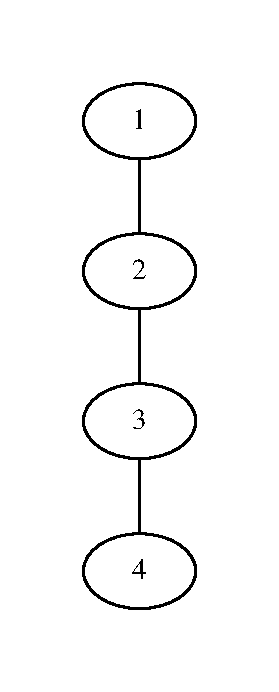
\includegraphics[scale=0.8]{kontrakt.pdf}
\end{subfigure}%
\begin{subfigure}{.5\textwidth}
	\centering
	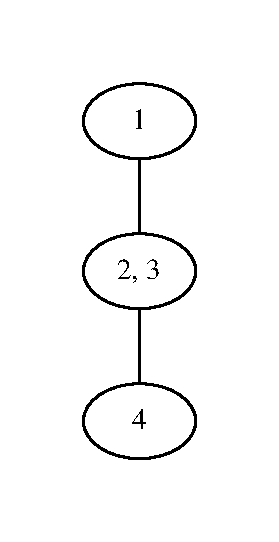
\includegraphics[scale=0.8]{kontrakt2.pdf}
\end{subfigure}
	\caption{Links: Der Graph $G = \left(
			\left\{1, 2, 3, 4\right\}, 
		\left\{
			\left\{\left\{1, 2\right\}\right\},
			\left\{\left\{2, 3\right\}\right\},
			\left\{\left\{3, 4\right\}\right\}
		\right\}
	\right)$. Rechts der kantenkontraktierte Graph $G' = \left(
		\left\{1, \text{\frq} 2, 3\text{\flq}, 4\right\}
		\left\{
			\left\{\left\{1, \text{\frq} 2, 3\text{\flq}\right\}\right\},
			\left\{\left\{\text{\frq} 2, 3\text{\flq}, 4\right\}\right\}
		\right\}
	\right)$.}
\label{kontraktiertergraph}
\end{figure}

\subsubsection{Gradmatrix}

\label{gradmatrix}

\picturetext{
Die Gradmatrix eines Graphen besteht aus Einträgen in der Hauptdiagonale, die 
je den Grad des Knoten bestimmen. Betrachten wir dazu den Stern $S_4$ auf der linken Seite.

Dieser besitzt die Gradmatrix:

\begin{equation}
	G = \begin{array}{r|c}
	& \begin{matrix} 1 & 2 & 3 & 4 \end{matrix} \\
	  \hline
	  \begin{matrix}
			1\\
			2\\
			3\\
			4\\
		\end{matrix} &
		\begin{pmatrix*}
			3 & 0 & 0 & 0\\
			0 & 1 & 0 & 0\\
			0 & 0 & 1 & 0\\
			0 & 0 & 0 & 1\\
		\end{pmatrix*}
	\end{array}
\end{equation}

Knoten $1$ ist das Zentrum des Sterns.}{\centering \stargraph{3}{2}}


\subsubsection{Adjazenzmatrix}

\label{adjazenzmatrix}

Die Adjazenzmatrix ist eine Möglichkeit, lineare Algebra und Graphentheorie zu verbinden. In einer solchen Adjazenzmatrix 
stellt man eine Tabelle auf, die alle Knoten $V(G)$ beinhaltet und setzt den Wert an der $(x, y)$-Spalte auf $1$, wenn die
Knoten eine gemeinsame Kante ($\left(\left(x_1, x_2\right) \in V(G)\right) \wedge \left(\left(x_1, x_2\right) \in E(G) \longrightarrow 1\right)$) haben und auf $0$, wenn nicht.

\begin{equation}
	\begin{array}{r|c}
	  & \begin{matrix} a & b & c \end{matrix} \\
	  \hline
	  \begin{matrix}
			a\\
			b\\
			c
		\end{matrix} &
		\begin{pmatrix*}
			0 & 1 & 0\\
			1 & 0 & 1\\
			0 & 1 & 0
		\end{pmatrix*}
	\end{array}
\end{equation}

\subsubsection{Cliquen}

Sei $G = (V, E)$ ein Graph. Dann ist $U$ eine Clique, wenn $U$ eine Untermenge von $V$ ist und alle Kanten von $U$ untereinander verbunden
sind.
Eine Clique heißt dann \textit{maximale Clique}, wenn man keine weiteren Kanten zu ihr hinzufügen kann und es trotzdem eine Clique
bleibt.

\subsubsection{Spannbäume}


Spannbäume --- auch: Gerüst --- sind Subgraphen, die ein Baum sind und alle Knoten
des Graphen enthalten (d.\,h. es werden nur Kanten entfernt).

Spannbäume von $G = \left\{\left\{a, b, c, d\right\}, \left\{
	\left\{a, c\right\},
	\left\{b, a\right\},
	\left\{c, d\right\},
	\left\{d, b\right\}
\right\}\right\}$.

\begin{tikzpicture}
	\begin{scope}[every node/.style={circle,thick,draw}]
		\node (a) at (-1,-1) {$a$};
		\node (b) at (1,-1) {$b$};
		\node (c) at (-1,1) {$c$};
		\node (d) at (1,1) {$d$};
	\end{scope}

	\begin{scope}[>={Stealth[black]}]
		\path (a) edge node {} (c);
		\path (b) edge node {} (a);
		\path (c) edge node {} (d);
		\path (d) edge node {} (b);
	\end{scope}
\end{tikzpicture}

\vspace{1cm}

\picturetext{
	\begin{tikzpicture}
		\begin{scope}[every node/.style={circle,thick,draw}]
			\node (a) at (-1,-1) {$a$};
			\node (b) at (1,-1) {$b$};
			\node (c) at (-1,1) {$c$};
			\node (d) at (1,1) {$d$};
		\end{scope}

		\begin{scope}[>={Stealth[black]}]
			\path (b) edge node {} (a);
			\path (c) edge node {} (d);
			\path (d) edge node {} (b);
		\end{scope}
	\end{tikzpicture}
}{
	\begin{tikzpicture}
		\begin{scope}[every node/.style={circle,thick,draw}]
			\node (a) at (-1,-1) {$a$};
			\node (b) at (1,-1) {$b$};
			\node (c) at (-1,1) {$c$};
			\node (d) at (1,1) {$d$};
		\end{scope}

		\begin{scope}[>={Stealth[black]}]
			\path (a) edge node {} (c);
			\path (c) edge node {} (d);
			\path (d) edge node {} (b);
		\end{scope}
	\end{tikzpicture}
}

\picturetext{
	\begin{tikzpicture}
		\begin{scope}[every node/.style={circle,thick,draw}]
			\node (a) at (-1,-1) {$a$};
			\node (b) at (1,-1) {$b$};
			\node (c) at (-1,1) {$c$};
			\node (d) at (1,1) {$d$};
		\end{scope}

		\begin{scope}[>={Stealth[black]}]
			\path (a) edge node {} (c);
			\path (b) edge node {} (a);
			\path (d) edge node {} (b);
		\end{scope}
	\end{tikzpicture}
}{
	\begin{tikzpicture}
		\begin{scope}[every node/.style={circle,thick,draw}]
			\node (a) at (-1,-1) {$a$};
			\node (b) at (1,-1) {$b$};
			\node (c) at (-1,1) {$c$};
			\node (d) at (1,1) {$d$};
		\end{scope}

		\begin{scope}[>={Stealth[black]}]
			\path (a) edge node {} (c);
			\path (b) edge node {} (a);
			\path (c) edge node {} (d);
		\end{scope}
	\end{tikzpicture}
}

\subsubsection{Satz von Kirchhoff}

Die Anzahl der Spannbäume eines Graphen kann mit dem Satz von Kirchhoff bestimmt
werden über die Determinante der \fullref{adjazenzmatrix} des Graphen.

Nehmen wir den Graphen $G = \left(
	\left\{1, 2, 3, 4\right\},
	\left\{
		\left\{
			1, 2
		\right\},
		\left\{
			1, 3
		\right\},
		\left\{
			3, 4
		\right\},
		\left\{
			2, 3
		\right\},
		\left\{
			2, 4
		\right\}
	\right\}
\right)$ als Beispiel.


\begin{tikzpicture}
	\begin{scope}[every node/.style={circle,thick,draw}]
		\node (eins) at (-1,-1) {$1$};
		\node (zwei) at (1,-1) {$2$};
		\node (drei) at (-1,1) {$3$};
		\node (vier) at (1,1) {$4$};
	\end{scope}

	\begin{scope}[>={Stealth[black]}]
		\path (eins) edge node {} (zwei);
		\path (eins) edge node {} (drei);
		\path (drei) edge node {} (vier);
		\path (zwei) edge node {} (drei);
		\path (zwei) edge node {} (vier);
	\end{scope}
\end{tikzpicture}

Erzeugen wir als erstes die Adjazenzmatrix 

\begin{equation}
	A = \begin{array}{r|c}
		& \begin{matrix} 1 & 2 & 3 & 4 \end{matrix} \\
	  \hline
	  \begin{matrix}
			1\\
			2\\
			3\\
			4
		\end{matrix} &
		\begin{pmatrix*}
			0 & 1 & 1 & 0 \\
			1 & 0 & 1 & 1 \\
			1 & 1 & 0 & 1 \\
			0 & 1 & 1 & 0 \\
		\end{pmatrix*}
	\end{array}.
\end{equation}

Nun bestimmen wir die \fullref{gradmatrix}:

\begin{equation}
	B = \begin{array}{r|c}
		& \begin{matrix} 1 & 2 & 3 & 4 \end{matrix} \\
	  \hline
	  \begin{matrix}
			1\\
			2\\
			3\\
			4
		\end{matrix} &
		\begin{pmatrix*}
			2 & 0 & 0 & 0 \\
			0 & 3 & 0 & 0 \\
			0 & 0 & 3 & 0 \\
			0 & 0 & 0 & 2 \\
		\end{pmatrix*}
	\end{array}.
\end{equation}

Daraus lässt sich die sogenannte Laplace-Matrix berechnen:

\begin{equation}
	L = B - A
\end{equation}

\begin{equation}
	L = \begin{pmatrix*}
		2 & 0 & 0 & 0 \\
		0 & 3 & 0 & 0 \\
		0 & 0 & 3 & 0 \\
		0 & 0 & 0 & 2 \\
	\end{pmatrix*} - \begin{pmatrix*}
		0 & 1 & 1 & 0 \\
		1 & 0 & 1 & 1 \\
		1 & 1 & 0 & 1 \\
		0 & 1 & 1 & 0 \\
	\end{pmatrix*} = \begin{pmatrix*}
		2 & -1 & -1 & 0 \\
		-1 & 3 & -1 & -1 \\
		-1 & -1 & 3 & -1 \\
		0 & -1 & -1 & 2\ \
	\end{pmatrix*}.
\end{equation}

Aus dieser Matrix lassen sich nun je eine beliebige Zeile und Spalte löschen, z.\,B.
\begin{equation}
	L* = \begin{pmatrix*}
		3 & -1 & -1 \\
		-1 & 3 & -1 \\
		-1 & -1 & 2\ \
	\end{pmatrix*}.
\end{equation}

Von dieser Matrix können wir nun die \fullref{determinante} bilden:

\begin{equation}
	\det\begin{pmatrix*}
		3 & -1 & -1 \\
		-1 & 3 & -1 \\
		-1 & -1 & 2\ \
	\end{pmatrix*} = 8.
\end{equation}

Wir erhalten $8$, und $8$ ist die Anzahl der Spannbäume des Graphen $G$.

\subsubsection{Satz von Cayley}

\label{cayley}

Der Satz von Cayley besagt, dass es $n^{n-2}$ verschiedene bezeichnete Bäume mit $n$ Knoten gibt. Dies kann unter Anderem
bewiesen werden durch die \fullref{pruefercodes}.

\subsubsection{Prüfer-Codes}

\label{pruefercodes}

Prüfer-Codes sind eine Methode, einen Baum eineindeutig mit einer Ziffernfolge zu beschreiben. Das heißt, dass jeder
Baum einen spezifischen Prüfer-Code hat und aus jedem Prüfer-Code ein spezifischer Baum wiederhergestellt werden kann.
Der Prüfer-Code eines Baumes mit $n$ Knoten hat $n - 2$ Zeichen, was den \fullref{cayley} beweist.

Zum Erstellen des Prüfer-Codes wählt man sich einen beliebigen Baum und schaut sich die einzelnen Blätter an. Es wird
das Blatt entfernt, das den geringsten Wert in der Beschriftung hat und in den Code der Wert des Knoten, an dem das
Blatt hängt, geschrieben. Dies wird iterativ fortgeführt, bis nur noch zwei Knoten übrig sind.

Beispiel.

\begin{tikzpicture}
	\begin{scope}[every node/.style={circle,thick,draw}]
		\node (a) at (0,0) {$1$};
		\node (b) at (-1,-1) {$2$};
		\node (c) at (1,-1) {$3$};
		\node (d) at (2,-2) {$4$};
	\end{scope}

	\begin{scope}[>={Stealth[black]}]
		\path (a) edge node {} (c);
		\path (b) edge node {} (a);
		\path (c) edge node {} (d);
	\end{scope}
\end{tikzpicture}

Die Blätter dieses Baumes sind $2, 4$. Das Blatt mit der geringsten Beschriftung
ist die $2$. Also entfernen wir die $2$ und schreiben die $1$, an der die $2$ hängt,
in den Prüfercode.

\begin{tikzpicture}
	\begin{scope}[every node/.style={circle,thick,draw}]
		\node (a) at (0,0) {$1$};
		\node (c) at (1,-1) {$3$};
		\node (d) at (2,-2) {$4$};
	\end{scope}

	\begin{scope}[>={Stealth[black]}]
		\path (a) edge node {} (c);
		\path (c) edge node {} (d);
	\end{scope}
\end{tikzpicture}

Prüfer-Code: $2$.

Das nächstgeringste Blatt ist die $1$, also entfernen wir die $1$ und schreiben
die $3$ in den Prüfer-Code.

\begin{tikzpicture}
	\begin{scope}[every node/.style={circle,thick,draw}]
		\node (c) at (1,-1) {$3$};
		\node (d) at (2,-2) {$4$};
	\end{scope}

	\begin{scope}[>={Stealth[black]}]
		\path (c) edge node {} (d);
	\end{scope}
\end{tikzpicture}

Prüfer-Code: $2, 3$.

Nun sind nur noch die Knoten $3, 4$ übrig. Das heißt, der Algorithmus terminiert hier
und an den Prüfer-Code wird das leere Wort $\epsilon$ angehangen: $2, 3, \epsilon$.

Zur Rekonstruktion braucht man nun die Knotenmenge, $E(G) = \left\{1, 2, 3, 4\right\}$, 
und den Prüfer-Code. 

\TODO

\subsubsection{Planare Graphen}

Ein planarer Graph ist ein Graph, der sich auf einer Ebene zeichnen lässt, ohne dass sich Kanten überschneiden.
Ein Beispiel dafür ist (vereinfacht) das Straßennetz, solange Brücken und Tunnel nicht vorhanden sind. Ein anderes
Beispiel wäre der Graph von Flüssen, wenn soetwas wie das Wasserstraßenkreuz Minden nicht berücksichtigt wird.

\subsubsection{Minoren}

\label{minoren}

Ein Graph $H$ heißt Minor, wenn er aus dem Graphen $G$ durch \fullref{kantenkontraktion}
oder durch Weglassen von Kanten oder Knoten entsteht. Die Benennung von Kanten spielt
hier keine Rolle, so dass $H$ auch dann ein Minor von $G$ ist, wenn die Kantenmengen
beider Graphen disjunkt sind, sie sich aber isomorph verhalten.

\subsubsection{Satz von Kuratowski}

Der Satz von Kuratowski besagt, dass ein Graph exakt dann planar ist,
wenn er weder $K_5$ noch $K_{3,3}$ als Minoren (vgl. \fullref{minoren}) enthält


\picturetext{
	\begin{tikzpicture}
		\begin{scope}[every node/.style={circle,thick,draw}]
			\node (la) at (0,0) {};
			\node (lb) at (0,2) {};
			\node (lc) at (0,4) {};

			\node (ra) at (3,0) {};
			\node (rb) at (3,2) {};
			\node (rc) at (3,4) {};
		\end{scope}
		\begin{scope}[>={Stealth[black]}]
			\path (la) edge node {} (ra);
			\path (la) edge node {} (rb);
			\path (la) edge node {} (rc);

			\path (lb) edge node {} (ra);
			\path (lb) edge node {} (rb);
			\path (lb) edge node {} (rc);

			\path (lc) edge node {} (ra);
			\path (lc) edge node {} (rb);
			\path (lc) edge node {} (rc);
		\end{scope}
	\end{tikzpicture}
}{
	Der bipartite Graph (vgl. \fullref{bipartit}) $K_{3,3}$. Wenn durch Wegstreichung
	und Kantenkontraktion aus einem Graphen auf irgendeine Weise $K_{3,3}$ erzeugt
	werden kann, ist der Graph nicht planar.
}

\picturetext{
	Genauso verhält es sich mit dem Graphen $K_5$. Ist dieser irgendwie durch
	Kantenkontraktion oder Wegstreichung von Kanten oder Knoten aus einem Graphen
	$G$ erzeugbar ist, dann ist $G$ nicht planar.
}{
	\begin{tikzpicture}[bullet/.style={circle, fill, inner sep=2pt}]
		\foreach \lab [count=\c, 
		evaluate=\c as \ang using {18+72*\c}] 
		in {1, 2, 3, 4 ,5} {
			\node[bullet] (\c) at (\ang:10mm) {};
			\node at (\ang:14mm){$\lab$};
			\foreach \i in {1,...,\c} {
				\draw(\i)--(\c);
			}
		}
	\end{tikzpicture}
}

\subsubsection{Eulerscher Polyedersatz}

Der eulersche Polyedersatz besagt, dass bei zusammenhängenden planaren Graphen
folgende Formel gilt:

\begin{equation}
	|E(G)| - |V(G)| + f = 2
\end{equation}

Dabei beschreibt $|E(G)|$ die Anzahl der Knoten, $|V(G)|$ die Anzahl der Kanten
und $f$ die Anzahl der Fläche, die im Graph (inklusive der einheitlichen Fläche
außerhalb des Graphen) entstehen.

\begin{center}
	\begin{tikzpicture}
		\begin{scope}[every node/.style={circle,thick,draw}]
			\node (a) at (0,0) {$1$};
			\node (b) at (0,2) {$2$};
			\node (c) at (2,0) {$3$};
		\end{scope}
		\begin{scope}[>={Stealth[black]}]
			\path (a) edge node {} (b);
			\path (b) edge node {} (c);
			\path (c) edge node {} (a);
		\end{scope}
	\end{tikzpicture}
\end{center}

Es gibt in diesem Graph 3 Knoten ($|V(G) = 3$), 3 Kanten ($E(G) = 3$) und zwei
Flächen ($f = 2$). Es gilt also:

\begin{equation}
	\underbrace{\underbrace{3}_{|E(G)|} - \underbrace{3}_{|V(G)|}}_{= 0} + \underbrace{2}_{f} = 2.
\end{equation}

\subsubsection{Bipartite Graphen}
\label{bipartit}

Ein Graph heißt \frq bipartit\flq, falls sich seine Knotenmengen aufteilen lassen
in Partitionsklassen, so, dass zwischen den Knoten in den Partitionsklassen keine
Verbindungen bestehen.

\picturetext{
	\centering
	\begin{tikzpicture}
		\begin{scope}[every node/.style={circle,thick,draw}]
			\node (la) at (0,2) {$1$};
			\node (lb) at (0,1) {$2$};
			\node (lc) at (0,0) {$3$};
			\node (ld) at (0,-1) {$4$};

			\node (ra) at (2,2) {$5$};
			\node (rb) at (2,1) {$6$};
			\node (rc) at (2,0) {$7$};
			\node (rd) at (2,-1) {$8$};
		\end{scope}

		\begin{scope}[>={Stealth[black]}]
			\path (la) edge node {} (ra);
			\path (la) edge node {} (rb);
			\path (la) edge node {} (rc);
			\path (la) edge node {} (rd);

			\path (lb) edge node {} (ra);
			\path (lb) edge node {} (rb);
			\path (lb) edge node {} (rc);
			\path (lb) edge node {} (rd);

			\path (lc) edge node {} (ra);
			\path (lc) edge node {} (rb);
			\path (lc) edge node {} (rc);
			\path (lc) edge node {} (rd);

			\path (ld) edge node {} (ra);
			\path (ld) edge node {} (rb);
			\path (ld) edge node {} (rc);
			\path (ld) edge node {} (rd);
		\end{scope}
	\end{tikzpicture}
}{Im links gezeigten Graph entstehen zwei Partitionsklassen, nämlich $\{1, 2, 3, 4\}$
und $\{5, 6, 7, 8\}$, denn innerhalb dieser Partitionsklassen befinden sich keine
Verbindungen.}

\subsection{Partitionen}

Partitionierung einer Menge $M$ bedeutet, dass man alle möglichen Untermengen
bildet, die in-sich disjunkt sind (anders als die Potenzmengen, die nicht
disjunkt sein müssen).

Gegeben sei die Menge $M = \left\{a, b, c\right\}$. Von dieser lassen sich nun $|M|$ Arten von Partitionen bilden.

\begin{itemize}
	\item 1-Partitionen: $\left\{\left\{a, b, c\right\}\right\}$

	\item 2-Partitionen: $\left\{\left\{a\right\}, \left\{b, c\right\}\right\}$,
		$\left\{\left\{a, b\right\}, \left\{ c\right\}\right\}$,
		$\left\{\left\{a, c\right\}, \left\{b\right\}\right\}$
	\item 3-Partitionen: $\left\{\left\{a, b, c\right\}\right\}$.
\end{itemize}

Graphisch kann man sich die Partitionierung vorstellen als Möglichkeit, eine Menge
von $n$ Elementen in verschiedene (einander nicht überlappende) Gruppen einzuordnen.

Die Anzahl an möglichen Partitionen einer Menge lässt sich über die bell'schen Zahlen bestimmen. Die bell'sche Zahl lässt sich rekursiv berechnen über

\begin{equation}
	B_{n + 1} = \sum_{k = 0}^n \binom{n}{k} B_k.
\end{equation}


\subsection{Relationen}

Eine zweistellige Relation ist eine Menge $R$, die Untermenge des 
kartesischen Produktes von 
$A \times B$ ist. Das kartesische Produkt ist die Verbindung aller Elemente einer 
Menge mit den Elementen einer Anderen. Beispiel:

\begin{equation}
	A = \left\{1, 2, 3\right\}, B = \left\{a, b, c\right\}
\end{equation}

\begin{equation}
	A \times B = \left\{
		\left\{a, 1\right\}, \left\{a, 2\right\}, \left\{a, 3\right\},
		\left\{b, 1\right\}, \left\{b, 2\right\}, \left\{b, 3\right\},
		\left\{c, 1\right\}, \left\{c, 2\right\}, \left\{c, 3\right\}
	\right\}
\end{equation}

$R$ könnte z.\,B. in diesem Beispiel sein: $R = \left\{
	\left\{a, 1\right\}, \left\{b, 2\right\}, \left\{c, 3\right\}
\right\}$. Das würde bedeuten, dass $a$ in Relation zu $1$ steht, $b$ in Relation zu
$2$ und $c$ in Relation zu $3$.

\subsubsection{Äquivalenzrelationen}

Eine Äquivalenzrelation besitzt drei Eigenschaften:

\begin{itemize}
	\item Reflexivität
	\item Transitivität
	\item Symmetrie.
\end{itemize}

\subsubsection{Eigenschaften von Relationen}

\paragraph{Reflexivität} Eine Relation $R$ ist reflexiv, wenn gilt, dass $\forall x: xRx$. Gilt dies nicht, ist die Relation entweder irreflexiv (wenn $\forall x: \lnot xRx$), oder 
besitzt keine Reflexivitätseigenschaften (wenn für einige Elemente $xRx$ gilt, aber für andere nicht).
Ein Beispiel für Reflexivität ist die Relation kleiner-gleich, denn $\vdash \forall n \in \mathbb{M}: n \leq n$.

\paragraph{Transitivität} Eine Relation $R$ ist transitiv, wenn gilt: $xRy \wedge yRz \implies xRz$. Das Gleichheitszeichen z.\,B. ist transitiv, denn
es gilt: $x = y \wedge y = z \implies x = z$. Das Gegenteil von Transitivität ist die Intransitivität, diese findet man z.\,B. beim Schnick-Schnack-Schnuck-Spiel,
denn $a$ schlägt $b$ ($aRb$), $b$ schlägt $c$ ($bRc$), aber $a$ schlägt $c$ nicht ($\not\vdash aRc$).

\paragraph{Symmetrie} Eine Relation $R$ ist symmetrisch, wenn $\forall x, y: xRy \longrightarrow yRx$. Beispiel für eine symmetrische Relation ist die Addition im
Ring $(\mathbb{N}, \cdot, +)$: dort gilt $a + b = b + a$ ($aRb \Leftrightarrow bRa$).

\subsubsection{Beispiel von Wikipedia}

Die Wikipedia liefert ein gutes Beispiel für eine Äquivalenzrelation.
Stellen wir uns eine Menge $T$ vor, die Tiere auf einem Bauernhof beinhaltet.
Wir definieren, dass $a, b, c \in T$ genau dann äquivalent sein sollen, wenn
$a$ und $b$ derselben Tierart angehören. 
Sind jetzt $a$ eine Kuh und $b$ ein Bulle, dann sind $a$ und $b$ in einer
Äquivalenzrelation, aber $c$ --- ein Hahn --- ist es nicht. Es gilt:

$a \sim b \wedge a \not\sim c$.

Hier sind alle drei Eigenschaften erfüllt:

\begin{itemize}
	\item Reflexivität: jedes Tier gehört zur selben Spezies wie es selbst
	\item Symmetrie: Seien $x, y, z$ Tiere aus $T$, dann gilt: wenn $x \sim y$ und
		$y \sim z$, dann ist auch $x \sim z$\footnote{Biologisch
		sind z.\,B. Ringspezies hiervon ausgeschlossen, aber wir gehen
		davon aus, dass der Bauernhof nicht genügend Zeit hatte, um
		ausreichend große evolutionäre Änderungen einzuführen.}
	\item Transitivität: wenn $a, b \in T: a \sim b$ ($a$ und $b$ gehören
		zur selben Spezies) und $c \in T: a \sim c$, dann gilt auch,
		dass $a$ und $c$ in der selben Spezies sind.
\end{itemize}

Die Äquivalenzklassen bestehen in diesem Beispiel aus den Tieren je einer Art.
Z.\,B. gehören Kuh und Bulle zur selben Äquivalenzklasse, Hahn und Huhn auch, aber
Hahn und Huhn und Kuh und Bulle sind nicht die gleichen Äquivalenzklassen.

\subsection{Ordnungen}

\subsubsection{Halbordnungen}

Eine Halbordnung besteht auf einer Menge $M$, wenn für alle Elemente $x, y \in M$
gilt:

\begin{itemize}
	\item $xRx$ (Reflexivität),
	\item $xRy \wedge yRx \implies x = y$ (Antisymmetrie),
	\item $xRy \wedge yRz \implies xRz$ (Transitivität).
\end{itemize}

Beispiel für eine Halbordnung ist der Teilerverband einer Zahl. In diesem
werden alle Teiler einer Zahl untereinander in Relation gesetzt. So sind
die Teiler von 
$\mathcal{T}(60) = \left\{1, 2, 3, 4, 5, 6, 10, 15, 30, 20, 12, 60\right\}$ 
ein Teilerverband und eine Halbordnung, da für alle $x, y \in \mathcal{T}$ gilt:

\begin{itemize}
	\item $x$ ist Teiler von $x$ (Reflexivität, jede natürliche Zahl teilt sich
		selbst),
	\item Wenn $x$ $y$ teilt und $y$ $x$ teilt, dann ist $x = y$ (Antisymmetrie)
	\item Wenn $x$ $y$ teilt und $y$ $z$ teilt, dann teilt auch 
		$x$ $z$ (Transitivität)
\end{itemize}

\subsubsection{Hasse-Diagramme}


\begin{wrapfigure}{r}{6cm}
	\centering
	\begin{tikzpicture}
		\node (max) at (0,2) {$70$};
		\node (a) at (-1,1) {$10$};
		\node (b) at (0,1) {$14$};
		\node (c) at (1,1) {$35$};
		\node (d) at (-1,0) {$2$};
		\node (e) at (0,0) {$5$};
		\node (f) at (1,0) {$7$};
		\node (min) at (0,-1) {$1$};
		\draw (min) -- (d) -- (a) -- (max) -- (b) -- (f)
		(e) -- (min) -- (f) -- (c) -- (max)
		(d) -- (b);
		\draw[preaction={draw=white, -,line width=6pt}] (a) -- (e) -- (c);
	\end{tikzpicture}
	\caption{Hasse-Diagramm des Teilerverbandes von 70}
	\label{hasse}
\end{wrapfigure}

Hasse-Diagramme sind eine Möglichkeit, Halbordnungen mithilfe eines
gerichteten Graphen darzustellen. 

Das Hasse-Diagramm vom Teilerverband der Teiler von 70 (mit 
$\mathcal{T}(70) = \left\{1, 2, 5, 7, 10, 14, 35, 70\right\}$) sich darstellen als
Graph (siehe dazu Abbildung \ref{hasse}).

Dabei werden zwei Knoten $a, b \in M$ verbunden, wenn gilt: $aRb$ (d.,\,h. wenn
gilt, dass $a, b$ transitiv, reflexiv und antisymmetrisch sind). 

In der Darstellung
des Hasse-Diagramms werden die Schleifen, die sich aus der Reflexivität ($aRa$ bzw.
in der Teilbarkeitsrelation $a$ teilt $a$, was für alle $a \in \mathbb{N}$ gilt) 
ergeben, weggelassen.

\subsubsection{Quasiordnungen}

Quasiordnungen sind reflexive und transitive Ordnungen, die aber nicht symmetrisch 
sein müssen (d.\,h. entweder symmetrisch, antisymmetrisch oder asymmetrisch). Jede
Äquivalenzrelation ist eine Quasiordnung mit Symmetrie.

Für eine Quasiordnung von $M$ gilt daher für alle $a, b, c \in M$:

\begin{itemize}
	\item $aRa$ (jedes Element steht mit sich selbst in der Relation 
		$R$, Reflexivität)
	\item $aRb \wedge bRc \implies aRc$ (Transitivität)
\end{itemize}

Ein Beispiel für eine Quasiordnung ist die Relation der Teilbarkeit auf
der Menge der natürlichen Zahlen, denn:

\begin{itemize}
	\item Jede natürliche Zahl ist durch sich selbst teilbar (Reflexivität)
	\item Wenn eine natürliche Zahl $a$ durch $b$ teilbar ist, und $b$ durch
		$c$, dann ist auch $a$ durch $c$ teilbar
\end{itemize}


\section{Lineare Algebra}

\subsection{Komplexe Zahlen}

Komplexe Zahlen ($\mathbb{C}$) erweitern die reellen Zahlen um die Möglichkeit, Gleichungen
der Struktur $x^2 + 1 = 0$ zu lösen, indem sie definieren, dass $i = \sqrt{-1}$ und folglich
$i^2 = -1$ zulässige Zahlen sind.

\subsubsection{Division komplexer Zahlen}

Für die Division durch komplexe Zahlen kann man einen Trick anwenden:

\begin{equation}
	\frac{a}{1 + i} = \frac{a}{1 + i} \cdot \frac{1 - i}{1 - i} =
	\frac{a \cdot (1 + i)}{(1 - i)(1 - i)} = 
	\frac{a \cdot (1 - i)}{2}.
\end{equation}

Dabei bildet man die komplex-konjugierte komplexe Zahl (Vorzeichenwechsel beim Imaginäranteil) und multipliziert sie sowohl im
Zähler als auch im Nenner an die Zahl. Das geht, weil sich dadurch die Relation nicht verändert (sie könnten ja jederzeit
wieder rausgestrichen werden). Der Vorteil ist, dass man die imaginäre Zahl damit aus dem 
Nenner herauskriegen kann.

\subsubsection{Addition in den komplexen Zahlen}

Die Addition in $\mathbb{C}$ geschieht komponentenweise, d.\,h.

\begin{equation}
	(a + bi) + (c + di) = (a+c) + ((b+d)i).
\end{equation}

\subsubsection{Gaußsche Zahlenebene}

\begin{figure}[h!]
	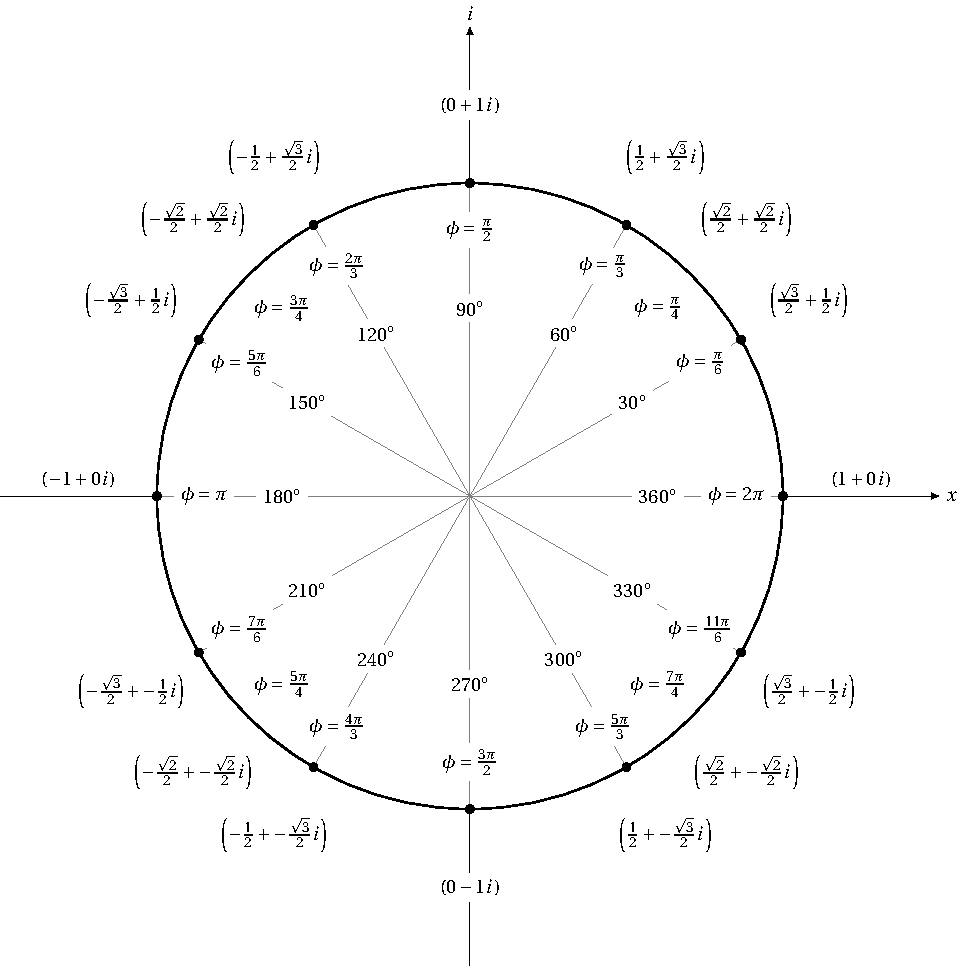
\includegraphics[width=\textwidth]{unit.pdf}
	\caption{Der Einheitskreis und einige komplexe Zahlen auf ihm.}
\end{figure}

Anstatt sich -- wie bei allen Zahlenklassen bis einschließlich $\mathbb{R}$ -- die Zahlen als geordnet in einer Linie vorzustellen,
bestimmen sich komplexe Zahlen durch ihre Position auf einer zweidimensionalen Fläche, der gauß'schen Zahlenebene.

Zahlen können hier über drei Schreibweise exakt verortet werden.

\begin{enumerate}
	\item $a + bi$, als cartesische Koordinaten
	\item $r \cdot e^\phi$, als Winkel $\phi$, der sich gegen den Uhrzeigersinn von der Reellen Achse abhebt und einen Abstand
		von $r$ hat,
	\item Als Sinus-Cosinusdarstellung: $r (\cos(\phi) + i\cdot\sin(\phi)$
\end{enumerate}

Wichtig zu merken ist für die letzten beiden Arten der Darstellung, dass $\pi$ eine halbe Umdrehung ist, so dass $2\pi$ eine ganze ist
und $\frac{\pi}{2}$ eine Viertelumdrehung. Darüber kann man oft optisch gut abschätzen, wo sich die Zahl befindet.

\subsubsection{Umrechnen in andere Darstellungsformen}

Für einige Operationen eignen sich andere Darstellungsformen einer komplexen Zahl besser als Andere. Daher kurz die Umrechnungsregeln:

\begin{tabular}{|l|l|}
	Variablenname & Bedeutung\\ \hline
	$\Im(z)$ & Imaginäranteil von z (bei $z = 4 + 6i$ ist $\Im(z) = 6$) \\
	$\Re(z)$ & Realanteil von z (bei $z = 4 + 6i$ ist $\Re(z) = 4$) \\
	$r$ & Der Abstand zum Nullpunkt auf kürzestem Wege \\
	$\phi$ & Der Winkel zur Achse der reellen Zahlen\\
\end{tabular}

\begin{equation}
	r = |z| = \sqrt{a^2 + b^2}
\end{equation}

\begin{equation}
	\sin(\phi) = \frac{y}{r}, 
	\cos(\phi) = \frac{x}{r}
\end{equation}

Mithilfe des Arcus-Sinus oder Arcus-Cosinus können wir dann die Werte für $\phi$ bestimmen. Jedoch ist es sehr hilfreich,
das geometrisch zu verstehen, denn häufig sind $\phi$-Werte gebrochen-rationale oder ganzzahlige Vielfache von $\pi$ (einer halben Drehung).

\subsubsection{Multiplikation komplexer Zahlen}

Wenn man zwei komplexe Zahlen multiplizieren will, z.\,B. $z_1 = 1 + 0i$ und $z_2 = 0 + 1i$, dann ist es einfacher,
sie in die $e$-Funktionsschreibweise zu bringen.

\begin{equation}
	z_1 = 1 + 0i = 1 \cdot e^{0\cdot \phi \cdot i} = 1 \cdot e^{0\cdot i} = 1
\end{equation}

\begin{equation}
	z_2 = 0 + 1i = 1 \cdot e^{1\cdot \frac{1}{2}\pi \cdot i} = e^{\frac{1}{2}\pi \cdot i}
\end{equation}

Wir erhalten dann:

\begin{equation}
	e^{0\cdot i} \cdot e^{\frac{1}{2}\pi \cdot i} = 
	e^{(0 \cdot i) + (\frac{1}{2}\pi \cdot i)} =
	e^{\frac{1}{2}\pi \cdot i}
\end{equation}

Durch das $\frac{1}{2}\pi$ kriegen wir eine Viertelkreisdrehung und landen exakt auf $i$, ohne Stauchung oder Streckung durch Vorfaktoren. 
Daher ist $z_1 \cdot z_2 = i$.

\subsubsection{Komplexe Potenzen}

\begin{equation}
	z = re^{i\phi},
\end{equation}
\begin{equation*}
	z^n = \left(re^{i\phi}\right)^n,
\end{equation*}
dank \fullref{warumxhochn} können wir schlussfolgern:
\begin{equation*}
	z^n = r^n \cdot e^{n\cdot i\phi}.
\end{equation*}

\subsubsection{Komplexe Wurzeln}

Komplexe Zahlen haben, im Gegensatz zu reellen, keine eineindeutige Wurzel mehr.

Wollen wir herausfinden, welche $z$ eingesetzt werden können, damit $z^5 = 1$ ist (d.\,h. wir wollen wir fünfte Wurzel ziehen),
dann müssen wir $z$ erst in die eulersche Form umwandeln, i.\,e. $z = r\cdot e^{\phi \cdot i}$.

Für $z^n$ sind die Wurzeln: $\sqrt[n]{r_0} \cdot e^{i \cdot \frac{\phi}{n} + \frac{2\pi}{n}\cdot k}$ für $k \in \{0, 1, 2, \dots, n - 1\}$.

\subsection{Matrixrechnung}

\subsubsection{Standardskalarprodukt}

Das Standardskalarprodukt von zwei Vektoren bestimmt sich aus der Summe der jeweiligen Zeilen, die multipliziert werden. Man kann schreiben:

\begin{equation}
	A^{1\times m} \cdot B^{1 \times m} = \sum_{i = 1}^{m} A_i \cdot B_i.
\end{equation}

Ein Beispiel:

\begin{equation}
	\begin{pmatrix*}
		a \\
		b \\
		c \\
	\end{pmatrix*} \cdot 
	\begin{pmatrix*}
		d \\
		e \\
		f \\
	\end{pmatrix*} = ab + be + cf.
\end{equation}

\subsubsection{Skalarmultiplikation}

Matrizen werden skalar multipliziert, indem der Vorfaktor (hier $a$) an jeden einzelnen Wert
heranmultipliziert wird:

\begin{equation}
	a \cdot \begin{pmatrix*}
		x_1 & y_1 & z_1\\
		x_2 & y_2 & z_2\\
	\end{pmatrix*} = \begin{pmatrix*}
		ax_1 & ay_1 & az_1\\
		ax_2 & ay_2 & az_2\\
	\end{pmatrix*}.
\end{equation}

Diese Relation lässt sich auch umkehren, um Matrizen zu vereinfachen, indem man gemeinsame Vorfaktoren herauszieht.

\subsubsection{Matrixmultiplikation}

Matrixmultiplikation funktioniert nur bei einigen Matrizen. Dabei kann nur eine $n\times m$-Matrix mit einer
$m\times n$-Matrix multipliziert werden. Die Matrixmultiplikation ist \textbf{nicht} kommutativ, d.\,h. im
allgemeinen Fall: $A \times B \not= B\times A$.

Matrizen werden multipliziert durch einen \frq Trick\flq. Man stelle sich vor, man nehme sich die $a$-te Spalte aus
der zweiten Matrix, kippe sie nach links zur Seite und lege sie über die $b$-te Spalte der ersten Matrix.
Multipliziert man diese nun miteinander und komponiert sie per Addition, dann ergibt sich der Wert an Position $(a, b)$
in der Ergebnismatrix.

Beispiel.

\begin{equation}
	\begin{pmatrix*}
		a & b & c\\
		d & e & f\\
	\end{pmatrix*} \cdot \begin{pmatrix*}
		h & i\\
		j & k\\
		l & m\\
	\end{pmatrix*} = \begin{pmatrix*}
		ah+bj+cl & ai+bk+cm\\
		dh+ej+fl & di+ek+fm\\
	\end{pmatrix*}.
\end{equation}

\subsubsection{Matrixaddition}

Bei einer Matrixaddition werden einfach alle komponenten an den Positionen $\langle a, b\rangle$ in beiden Matrizen addiert.
Dabei müssen die beiden Matrizen gleichen Types sein, d.\,h. $A^{n\times n} \wedge B^{n\times n}$.

Beispiel:

\begin{equation}
	\begin{pmatrix*}
		a & b & c\\
		d & e & f\\
	\end{pmatrix*} + \begin{pmatrix*}
		h & i & j\\
		k & l & m\\
	\end{pmatrix*} = \begin{pmatrix*}
		a+h & b+i & c+j\\
		d+k & e+l & f+m\\
	\end{pmatrix*}
\end{equation}

\subsubsection{Determinante}

\label{determinante}

Die Determinante einer Matrix bestimmt im Zusammenhang mit der linearen Algebra die Flächen- bzw. Volumenveränderung einer
Struktur, wenn man sie anhand dieser Matrix manipuliert.

Die Determinante der Matrix \begin{equation}
	A \in K^{2\times 2} = \begin{pmatrix*}
		a & b\\
		c & d\\
	\end{pmatrix*}
\end{equation}
bestimmt sich als $ad - bc$.

Für quadratische Matrizen bis $3\times 3$ lässt sich die Determinante durch die Regel von Sarrus bestimmen, in der man (wie in der Abbildung) pfeilweise multipliziert
und dann die Produkte addiert bzw. subtrahiert.

\begin{equation}
	\det(A)=\begin{pmatrix*} a & b & c \\ d & e & f \\ g & h & i \end{pmatrix*} = \begin{pmatrix*}
		\begin{tikzpicture}
			\matrix [
				matrix of math nodes,
				column sep=1em,
				row sep=1em
				] (sarrus) {
					a & b & c & a & b \\ d & e & f & d & e\\ g & h & i & g & h\\
					};

					\path ($(sarrus-1-3.north east)+(0.5em,0)$) edge[thick,dotted] ($(sarrus-3-3.south east -| sarrus-1-3.north east)+(0.5em,0)$);
					% \path ($(sarrus-1-4.north west)-(0.5em,0)$) edge[thick,dotted] ($(sarrus-3-4.south west)-(0.5em,0)$);
					\path[->,blue] (sarrus-1-1) edge (sarrus-2-2)
					(sarrus-2-2) edge (sarrus-3-3)
					(sarrus-1-2) edge (sarrus-2-3)
					(sarrus-2-3) edge (sarrus-3-4)
					(sarrus-1-3) edge (sarrus-2-4)
					(sarrus-2-4) edge (sarrus-3-5);

					\path[->,red](sarrus-3-1) edge[dashed] (sarrus-2-2)
					(sarrus-2-2) edge[dashed] (sarrus-1-3)
					(sarrus-3-2) edge[dashed] (sarrus-2-3)
					(sarrus-2-3) edge[dashed] (sarrus-1-4)
					(sarrus-3-3) edge[dashed] (sarrus-2-4)
					(sarrus-2-4) edge[dashed] (sarrus-1-5);

					\foreach \c in{3,4,5} \node[blue] at (sarrus-3-\c.south east) {$+$};
					\foreach \c in{3,4,5} \node[red] at (sarrus-1-\c.north east) {$-$};
		\end{tikzpicture}
\end{pmatrix*} = 
aei + bfg + cdh - gec - hfa - idb.
\end{equation}

Wenn die Determinante einer Matrix ungleich 0 ist, dann ist die Matrix invertierbar (vgl. \fullref{invertieren}).

Für größere quadratische Matrizen lässt sich die Determinante über den sogenannten \frq Laplace'schen Entwicklungssatz\flq\ entwickeln.

Wir wählen dazu eine beliebige Zeile aus (im einfachsten Fall eine, in der möglichst viele Nullen vorkommen) und gehen sie elementweise
durch. Die Zeile und Spalte, in der sie sich befindet, blenden wir in Gedanken aus, und berechnen aus den übriggebliebenen Spalten und
Zeilen die Determinante. Diese multiplizieren wir nun mit dem Wert aus der ausgeblendeten Spalte und addieren sie
alternierend (beginnend mit $+$). Das Ergebnis ist die Determinante der Matrix.

\begin{equation}
	\det\begin{pmatrix*}
		a & b & c \\
		d & e & f \\
		g & h & i \\
	\end{pmatrix*} =
\end{equation}
\begin{equation}
	a \cdot \det\begin{pmatrix*}
		\mystar & \mystar & \mystar \\
		\mystar & e	  & f \\
		\mystar & h       & i \\
	\end{pmatrix*} - b \cdot \det\begin{pmatrix*}
		\mystar & \mystar & \mystar \\
		d       & \mystar & f \\
		g       & \mystar & i \\
	\end{pmatrix*} + c \cdot \det\begin{pmatrix*}
		\mystar & \mystar & \mystar \\
		d       & e       & \mystar \\
		g       & h       & \mystar \\
	\end{pmatrix*} = 
\end{equation}
\begin{equation}
	a\cdot \det\begin{pmatrix*}
		e & f \\
		h & i \\
	\end{pmatrix*} - b\cdot \det\begin{pmatrix*}
		d & f \\
		g & i \\
	\end{pmatrix*} + c\cdot \det\begin{pmatrix*}
		d & e \\
		g & h \\
	\end{pmatrix*} =
\end{equation}
\begin{equation}
	a(ei - hf) - b(di - gf) + c(dh - ge) = 
	aei - ahf  - bdi + bgf  + cdh - cge
\end{equation}

Matrizen der Form $\mathbb{K}^{n\times n}$ können hiermit in Matrizen der Form $\mathbb{K}^{n - 1 \times n - 1}$ \frq heruntergebrochen\flq\ werden. 
Damit lassen sich prinzipiell rekursiv alle quadratischen Matrizen determinieren, wenn man dieses Verfahren dann auf die 
$n - 1 \times n - 1$-Matrix anwendet, bis man viele kleine $2 \times 2$-Matrizen hat, die über die Formel
$\det\begin{pmatrix*}
	a & b \\
	c & d \\
\end{pmatrix*} = ad - cb$ berechnet werden können.



\subsubsection{Die Zeilenstufenform}

\label{zeilenstufenform}
Jede Matrix kann durch Operationen auf sie in die Zeilenstufenform überführt werden. Dazu sind zwei
Begriffe relevant:

\begin{tabular}{|l|l|}
	\hline
	Begriff & Erklärung\\ \hline
	Nullzeile & Eine Zeile, in der nur Nullen stehen\\
	Zeilenführer & Erste Zahl in einer Zeile, die nicht $0$ ist\\
	\hline
\end{tabular}

Die Zeilenführer habe ich in dieser Beispielmatrix \textcolor{green}{grün} eingefärbt, die 
Nullzeilen \textcolor{red}{rot}.

\begin{equation}
	\begin{pmatrix*}
		\textcolor{green}{1} & 0 & 1\\
		\textcolor{green}{2} & 0 & 4\\
		\textcolor{red}{0} & \textcolor{red}{0} & \textcolor{red}{0}\\
	\end{pmatrix*}
\end{equation}

Ziel ist es, dass der Zeilenführer von oben nach unten betrachtet von links nach rechts wandert und
eine \frq Treppe\flq\ entsteht\footnote{Mir hat es geholfen zu erkennen, dass die Treppe von Rechts nach
Links geht und nicht von Links nach Rechts.}.
Bei der Beispielmatrix erreicht man das mit 

\begin{equation}
	\begin{pmatrix*}
		\textcolor{green}{1} & 0 & 1\\
		\textcolor{green}{2} & 0 & 4\\
		\textcolor{red}{0} & \textcolor{red}{0} & \textcolor{red}{0}\\
	\end{pmatrix*} \xrightarrow{\ro{II} \rightarrow \ro{II} - 2\cdot \ro{I}} \begin{pmatrix*}
		\textcolor{green}{1} & 0 & 1\\
		0 & 0 & \textcolor{green}{2}\\
		\textcolor{red}{0} & \textcolor{red}{0} & \textcolor{red}{0}\\
	\end{pmatrix*}
\end{equation}

Legale Operationen sind dabei die Multiplikation mit Skalaren aus $\mathbb{R}$ und die Addition und Subtraktion von
Zeilen aus der Matrix selbst miteinander (z.\,B. die Zweite Zeile von der ersten abziehen oder addieren, d.\,h. Komponente-für-Komponente
durchgehen und voneinander abziehen oder addieren). Außerdem kann man die Zeilen beliebig vertauschen.

\subsubsection{Lösung linearer Gleichungssysteme mit Matrizen}

Ein lineares Gleichungssystem der Form 
\begin{equation}
	3x + 5y + z = 6
\end{equation}

\begin{equation}
	12x + 5z - 7z = 5
\end{equation}

\begin{equation}
	-x + y - 2z = -1
\end{equation}
kann mit einer erweiterten Koeffizientenmatrix dargestellt werden als:

\begin{equation}
	\left(
	\begin{array}{ccc|c}
		3 & 5 & 1 & 6\\
		12 & 5 & -6 & 5\\
		-1 & 1 & -2 & -1\\
	\end{array}
	\right)\begin{pmatrix*}
		x\\
		y\\
		z\\
	\end{pmatrix*}.
\end{equation}

Dadurch, dass man die Zeilenvektoren miteinander multipliziert und addiert und skalar multipliziert, kann man, wenn
das Gleichungssystem lösbar ist, eine Einsermatrix der Form
\begin{equation}
	\left(
	\begin{array}{ccc|c}
		1 & 0 & 0 & a\\
		0 & 1 & 0 & b\\
		0 & 0 & 1 & c\\
	\end{array}
	\right).
\end{equation}

Dann steht dort quasi $x = a, y = b$ und $z = c$.

\subsubsection{Matrixtransponierung}

Beim Transponieren einer Matrix wird die erste Zeile zur ersten Spalte, die zweite Spalte zur zweiten Zeile usw.

Beispiel:

\begin{equation}
	A^T = \begin{pmatrix*}
		1 & 2\\
		3 & 4\\
		5 & 6\\
	\end{pmatrix*}^T = \begin{pmatrix*}
		1 & 3 & 5\\
		2 & 4 & 6\\
	\end{pmatrix*}.
\end{equation}

Allgemeine Rechenregeln:

$$ (A^T)^T = A $$

$$ A^T + B^T = (A + B)^T $$

$$ (A \cdot B)^T = B^T \cdot A^T $$

\subsubsection{Spur}

Die Spur einer Matrix $K^{n\times n}$ ist die Summe ihrer Hauptdiagonalelemente.

Beispiel:

\begin{equation}
	\mathrm{Spur}\begin{pmatrix*}
		\textcolor{red}{a} & b & c & d \\
		e & \textcolor{red}{f} & h & h \\
		i & j & \textcolor{red}{k} & l \\
		m & n & o & \textcolor{red}{p} \\
	\end{pmatrix*} = a + f + k + p.
\end{equation}

Wenn die Spur einer Matrix $0$ ist, dann gilt die Matrix als spurfrei. 

Allgemein gilt: 

\begin{itemize}
	\item Die Spur einer Matrix ist gleich der Summe ihrer Eigenwerte.
	\item $\mathrm{Spur}(A) = \mathrm{Spur}(A^T)$
\end{itemize}

\subsubsection{Invertieren einer Matrix}

\label{invertieren}

Eine Matrix multipliziert mit ihrem Inversen ergibt die Einheitsmatrix. Beispiel:

\begin{equation}
	M = \begin{pmatrix*}
		2 & 5 \\
		1 & 3 \\
	\end{pmatrix*},
\end{equation}

\begin{equation}
	M \cdot M^{-1} = \begin{pmatrix*}
		1 & 0 \\
		0 & 1 \\
	\end{pmatrix*}.
\end{equation}

Die Methode dafür ist, die Matrix, in unserem Fall $M = \begin{pmatrix*}
	2 & 5 \\
	1 & 3 \\
\end{pmatrix*}$, mit der Einheitsmatrix als Koeffizientenmatrix aufzuschreiben. Wir haben dann also:

\begin{equation}
	M = \left(\begin{matrix}
		2 & 5 \\
		1 & 3 \\
	\end{matrix}
	\middle\vert
	\begin{matrix}
		1 & 0 \\
		0 & 1\\
	\end{matrix}\right).
\end{equation}

Nun stellen wir so lange um, bis wir links die Einheitsmatrix erhalten.

Zuerst schicken wir II auf $2\cdot$ II.

\begin{equation}
	M = \left(\begin{matrix}
		2 & 5 \\
		2 & 6 \\
	\end{matrix}
	\middle\vert
	\begin{matrix}
		1 & 0 \\
		0 & 2\\
	\end{matrix}\right).
\end{equation}

Dann schicken wir II auf II $ - $ I:

\begin{equation}
	M = \left(\begin{matrix}
		2 & 5 \\
		0 & 1 \\
	\end{matrix}
	\middle\vert
	\begin{matrix}
		1 & 0 \\
		-1 & 2\\
	\end{matrix}\right).
\end{equation}

Dann schicken wir I auf I $ - 5\cdot $ I:

\begin{equation}
	M = \left(\begin{matrix}
		2 & 0 \\
		0 & 1 \\
	\end{matrix}
	\middle\vert
	\begin{matrix}
		6 & -10 \\
		-1 & 2\\
	\end{matrix}\right).
\end{equation}

Dann schicken wir I auf $\frac{\mathrm{I}}{2}$:

\begin{equation}
	M = \left(\begin{matrix}
		1 & 0 \\
		0 & 1 \\
	\end{matrix}
	\middle\vert
	\begin{matrix}
		3 & -5 \\
		-1 & 2\\
	\end{matrix}\right).
\end{equation}

Im rechten Teil der Matrix können wir nun die invertierte Matrix ablesen.

Aus diesem Verfahren ist offensichtlich, dass sich nicht alle Matrizen invertieren lassen, denn hat man z.\,B. die Nullmatrix,
dann kann man die Zeilen so oft und viel miteinander verrechnen wie man will und man kommt nie zum Ende. Wenn alle Zeilen
linear abhängig sind, dann ist die Matrix nicht invertierbar, genauso, wenn die Determinante gleich 0 ist.

\subsubsection{Die Dimension einer Matrix}

\label{dimension}

Die Dimension einer Matrix bestimmt sich aus der Anzahl der linear unabhängigen Spalten der Matrix. Die Dimension einer Matrix bestimmt,
in wie vielen räumlichen Dimensionen sich ein Vektor, der ein Vielfaches der Matrix ist, ausbreiten kann.

Beispiel:

\begin{equation}
	U = \begin{pmatrix*}
		1 & 2 & 1 \\
		1 & 2 & -1 \\
		2 & 4 & 10 \\
	\end{pmatrix*} = \left\{\begin{pmatrix*}
		\begin{pmatrix*}
			1\\
			1\\
			2\\
		\end{pmatrix*} +
		2\times \begin{pmatrix*}
			1\\
			1\\
			2\\
		\end{pmatrix*} +
		\begin{pmatrix*}
			1\\
			-1\\
			10\\
		\end{pmatrix*}
	\end{pmatrix*}\right\}.
\end{equation}

Da der erste und zweite Vektor linear abhängig sind, fällt einer der beiden bei der Dimensionsbetrachtung weg. Daher gilt: $\textrm{Dim}\left(U\right) = 2$.
Wenn die Spaltenvektoren keien Vielfachen sind, dann müssen auch noch die Zeilenvektoren überprüft werden.

\subsubsection{Der Rang einer Matrix}

Der Rang bezeichnet die Anzahl der unabhängigen Zeilen- und Spaltenvektoren einer Matrix.

Die Matrix 
\begin{equation}
	A = \begin{pmatrix*}
		1 & 3 & -1\\
		2 & 6 & -2\\
		5 & 23 & 0\\
	\end{pmatrix*}, A \in \mathbb{N}^{3\times 3}
\end{equation}
hat die Zeilenvektoren
\begin{equation}
	\begin{pmatrix*}
		1 & 3 & -1\\
	\end{pmatrix*}, 
	\begin{pmatrix*}
		2 & 6 & -2\\
	\end{pmatrix*},
	\begin{pmatrix*}
		5 & 23 & 0\\
	\end{pmatrix*}
\end{equation}
und die Spaltenvektoren
\begin{equation}
	\begin{pmatrix*}
		1\\
		2\\
		5\\
	\end{pmatrix*},
	\begin{pmatrix*}
		3\\
		6\\
		23\\
	\end{pmatrix*},
	\begin{pmatrix*}
		-1\\
		-2\\
		0\\
	\end{pmatrix*}.
\end{equation}

Als erstes müssen wir versuchen, die Matrix in die Zeilenstufenform zu bringen (vgl. \fullref{zeilenstufenform}.

\begin{equation}
	\begin{pmatrix*}
		1 & 3 & -1\\
		2 & 6 & -2\\
		5 & 23 & 0\\
	\end{pmatrix*} \xrightarrow{\ro{II} \rightarrow 2\cdot \ro{I}} \begin{pmatrix*}
		1 & 3 & -1\\
		0 & 0 & 0\\
		5 & 23 & 0\\
	\end{pmatrix*} \xrightarrow{\ro{II} \leftrightarrow \ro{III}} \begin{pmatrix*}
		1 & 3 & -1\\
		5 & 23 & 0\\
		0 & 0 & 0\\
	\end{pmatrix*}
\end{equation}

Um die Zeilenstufenform zu vollenden, müssen wir nun nur noch den Zeilenführer der zweiten Zeile verschieben:

\begin{equation}
	\begin{pmatrix*}
		1 & 3 & -1\\
		5 & 23 & 0\\
		0 & 0 & 0\\
	\end{pmatrix*} \xrightarrow{\ro{II} \rightarrow \ro{II} - 5\cdot I} \begin{pmatrix*}
		1 & 3 & -1\\
		0 & 8 & 5\\
		0 & 0 & 0\\
	\end{pmatrix*}
\end{equation}

und wir haben die Zeilenstufenform. Der Rang der Matrix ist die Anzahl von Zeilen, die nicht ausschließlich aus 0 bestehen.
Das heißt: $\textrm{rang}(A) = 2$, weil von den drei Zeilen zwei nicht 0 sind.

\subsubsection{Der Kern einer Matrix}

Der Kern einer Matrix ist dadurch bestimmt, dass die Matrix multipliziert mit ihrem Kern zum Nullvektor wird. Das heißt abstrakt:
$\textrm{Ker}(A^{n\times m}) = \left\{x \in \mathbb{R}^{n\times 1} \middle| Ax = \vec{0}\right\}$.

Oder im konkreten Beispiel:

\begin{equation}
	U = \begin{pmatrix*}
		1 & 2 & 1 \\
		1 & 0 & -1 \\
		2 & 1 & 10 \\
	\end{pmatrix*},
\end{equation}

\begin{equation}
	\textrm{Ker}\left(U\right) \Rightarrow
	\begin{pmatrix*}
		1 & 2 & 1 \\
		1 & 0 & -1 \\
		2 & 1 & 10 \\
	\end{pmatrix*} \times \begin{pmatrix*}
		x_1 \\
		x_2 \\
		x_3 \\
	\end{pmatrix*} =
	\begin{pmatrix*}
		0\\
		0\\
		0\\
	\end{pmatrix*}
\end{equation}

Das impliziert die Gleichungssysteme:

\begin{equation}
	x_1 + 2x_2 + x_3 = 0
\end{equation}
\begin{equation}
	x_1 + \phantom{0x_2} - x_3= 0
\end{equation}
\begin{equation}
	2x_1 + x_2 + 10x_3 = 0
\end{equation}

Daraus ergibt sich, dass $x_1 = x_2 = x_3 = 0$. Das heißt, $\textrm{Ker}(U) = \begin{pmatrix*} 0\\
	0\\
	0\\
\end{pmatrix*}$. (Es ist der Nullvektor, weil alle Zeilen voneinander unabhängig waren; bei abhängigen Zeilen
gäbe es etwas Anderes als den Nullvektor.)

Die Dimension (vgl. \fullref{dimension}) des Kerns bestimmt sich durch die Anzahl linear unabhängiger Werte in ihr, d.\,h. für dieses 
Beispiel $\textrm{dim}\left(\textrm{Ker}\left(U\right)\right) = 1$, da alle Werte 0 sind und damit linear
abhängig voneinander.

\subsubsection{Multilinearität von Matrizen}

Gegeben sei die Matrix $M \in \mathbb{K}^{n\times n}$ mit:

\begin{equation}
	\begin{pmatrix*}
		a & b & c \\
		xd & xe & xf \\
		h & i & j \\
	\end{pmatrix*}
\end{equation}

und die Matrix $M'$ ohne den Vorfaktor $x$:

\begin{equation}
	\begin{pmatrix*}
		a & b & c \\
		d & e & f \\
		h & i & j \\
	\end{pmatrix*}
\end{equation}

Dann ist die Determinante $\det(M) = x \det(M')$.

Gleiches gilt für Spalten. So ist

\begin{equation}
	\det\begin{pmatrix*}
		a & xb & c \\
		d & xe & f \\
		h & xi & j \\
	\end{pmatrix*} = x\det\begin{pmatrix*}
		a & b & c \\
		d & e & f \\
		h & i & j \\
	\end{pmatrix*}.
\end{equation}

Ist ein Vorfaktor in jeder Zeile, wie z.\,B. ein \frq -\flq, dann kann man ihn auch \frq herausziehen\flq:

\begin{equation}
	\det(-M) = \det\begin{pmatrix*}
		-a & -b & -c \\
		-d & -e & -f \\
		-h & -i & -j \\
	\end{pmatrix*} = (-1)^3 \det\begin{pmatrix*}
		a & b & c \\
		d & e & f \\
		h & i & j \\
	\end{pmatrix*}.
\end{equation}

\subsubsection{Schnell Potenzen von Matrizen berechnen}

\TODO

\begin{equation}
	A = SDS^{-1}
\end{equation}


\subsection{Vektorräume und Untervektorräume}

\paragraph{Allgemeine Definition.} Sei $K$ ein Körper, dann ist $(V, +, \langle k | k \in K\rangle)$ ein K-Vektorraum.
Dieser besteht aus:
\begin{itemize}
	\item Einer Menge $V$, die ungleich der leeren Menge ist.
	\item Einer Addition: $+: V\times V \rightarrow V$.
	\item Einer Skalarmultiplikation $(k|k\in K): K\times V \rightarrow V$.
\end{itemize}

Beispiele für Vektorräume sind der allgemeine $K$-VR oder mit spezifischen Körpern
der $\mathbb{R}$-Vr oder $\mathbb{C}$-VR.

\subsubsection{Vektorraumaxiome}

\begin{enumerate}
	\item $\forall v_1, v_2 \in V$ ist $v_1 \times v_2$ ein eindeutig bestimmtes Element von $V$.
	\item $v_1, v_2, v_3 \in V: v_1 + (v_2 + v_3) = (v_1 + v_2) + v_3$ (Assoziativ)
	\item $v_1, v_2 \in V: v_1 + v_2 = v_2 + v_1$ (Kommutativ)
	\item $\forall v \in V: \exists \vec{0} \in V: v = \vec{0} + v = v + \vec{0}$ (Nullvektor als neutrales Element der Addition)
	\item $\forall v \in V: \exists -v \in V: v + (-v) = (-v) + v = \vec{0}$ (Jedes Element hat ein additives Inverses)
	\item $\forall k \in K: \forall v \in V: \exists kv \in V$
	\item $\forall v \in V: \vec{1}\cdot v = v$ (Einsvektor als neutrales Element der Multiplikation)
	\item $\forall k_1, k_2 \in K: \forall v \in V: (k_1k_2)v = k_2(k_1v)$ (Assoziativität der Multiplikation)
	\item $\forall k \in K: \forall v_1, v_2 \in V: (k_1 + k_2) \times v = vk_1 + vk_2$
	\item $\forall k \in K: \forall v_1, v_2 \in V: k(v_1 + v_2) = kv_1 + kv_2$
\end{enumerate}

\subsubsection{Bestimmen, ob $U$ ein Untervektorraum von $V$ ist}

Um zu bestimmen, ob $U$ ein Untervektorraum von $V$ ist, muss man schauen, ob der Nullvektor in diesem Vektorraum ist.
Das heißt, das Gleichungssystem

\begin{equation}
	U\times\vec{x} = \vec{0} =
	\begin{pmatrix*}
		a_1 & b_1 \\
		a_2 & b_2 \\
		a_3 & b_3 \\
	\end{pmatrix*} \times \begin{pmatrix*}
		x_1 \\
		x_2 \\
	\end{pmatrix*} = \begin{pmatrix*}
		0 \\
		0 \\
		0 \\
	\end{pmatrix*}
\end{equation}
muss Lösungen haben. Hat es keine, ist es kein Untervektorraum.

Hat es welche, muss weiterhin überprüft werden, ob man durch Addition oder Multiplikation aus dem Vektorraum herauskommt. Sollte
z.\,B. die Beschränkung sein, dass $a_n \leq 1 \wedge b_n \leq 1$, dann käme man mit einer Multiplikation, die $a$ oder $b$
größer $1$ machen würde, aus dem Vektorraum hinaus und $U$ wäre kein Untervektorraum.

Jeder Untervektorraum ist selbst wieder ein Vektorraum. Die anderen Axiome (z.\,B. die Assoziativität der Multiplikation) müssen
nicht überprüft werden. Diese werden vom Übervektorraum \frq geerbt\flq.

\subsubsection{Lineare Abhängigkeit}

\label{lineareabhaengigkeit}

Zwei Vektoren sind linear abhängig, wenn der eine ein Vielfaches des Anderen ist. So ist z.\,B.

\begin{equation}
	\begin{pmatrix*}
		1\\
		2\\
		3\\
	\end{pmatrix*} = \frac{1}{2} \times \begin{pmatrix*}
		2\\
		4\\
		6\\
	\end{pmatrix*}.
\end{equation}

Damit sind diese beiden Vektoren Vielfache voneinander und linear abhängig.

Die Vektoren $\begin{pmatrix*}
	0\\
	1\\
\end{pmatrix*}$ und $\begin{pmatrix*}
	1\\
	0\\
\end{pmatrix*}$ können beispielsweise nicht linear abhängig sein, denn die $0$ lässt sich durch keine Multiplikation
zu einer $1$ machen.

Ein effizienter Algorithmus zum Herausfinden, ob eine Menge von Vektoren Vielfache voneinander sind, wäre es, 
die einzelnen Vektoren $\vec{v_1}, \vec{v_2}, \dots, \vec{v_n}$ zu ordnen und anzufangen mit $\vec{v_1}$ und diesen
mit jedem $\vec{v_2}, \dots, \vec{v_n}$ zu vergleichen. Ist er ein Vielfaches von irgendeinem dieser Vektoren,
streichen wir ihn und brechen die Betrachtung für den ersten Vektor ab.
Dann \frq verschieben\flq\ wir das Raster und fangen mit $\vec{v_2}$ an und vergleichen ihn mit $\vec{v_3}, \dots, \vec{v_n}$,
streichen ihn raus, wenn er ein Vielfaches von einem dieser Vektoren ist und wiederholen dies, bis wir alle Vektoren einmal
miteinander verglichen haben.

Die nun nicht-durchgestrichenen Vektoren sind keine Vielfache voneinander.

\subsubsection{Span bestimmen}

Gegeben sei 
\begin{equation}
	U = \left\{\begin{pmatrix*}
		a + 3b - 8c \\
		a - b + 4c \\
		2a -b + 5c\\
	\end{pmatrix*}\middle| a, b, c \in \mathbb{R} \right\}.
\end{equation}

Diese lässt sich umschreiben zu:

\begin{equation}
	U = \left\{\begin{pmatrix*}
		a \\
		a \\
		2a \\
	\end{pmatrix*} + \begin{pmatrix*}
		3b \\
		-b \\
		-b \\
	\end{pmatrix*}+ \begin{pmatrix*}
		-8c \\
		4c \\
		5c \\
	\end{pmatrix*}
	\middle| a, b, c \in \mathbb{R} \right\}.
\end{equation}

Nun klammern wir die Parameter aus:

\begin{equation}
	U = \left\{a\times \begin{pmatrix*}
		1 \\
		1 \\
		2 \\
	\end{pmatrix*} + b\times \begin{pmatrix*}
		3 \\
		-1 \\
		-1 \\
	\end{pmatrix*}+ c\times \begin{pmatrix*}
		-8 \\
		4 \\
		5 \\
	\end{pmatrix*}
	\middle| a, b, c \in \mathbb{R} \right\}.
\end{equation}

Lassen wir nun die Parameter weg, erhalten wir fast den Span:

\begin{equation}
	\textrm{Span}_\mathbb{R}(U) = \textrm{Span}_\mathbb{R}\left(\left\{\begin{pmatrix*}
		1 \\
		1 \\
		2 \\
	\end{pmatrix*}, \begin{pmatrix*}
		3 \\
		-1 \\
		-1 \\
	\end{pmatrix*}, \begin{pmatrix*}
		-8 \\
		4 \\
		5 \\
	\end{pmatrix*}
	\right\}\right).
\end{equation}

Der einzige Schritt, den wir jetzt noch checken müssen ist, ob die Parameter linear abhängig sind oder nicht (vgl. auch \fullref{lineareabhaengigkeit}).
Aus der Menge der untereinander linear abhängigen Parameter muss dann noch einer ausgewählt werden (welcher ist egal, denn sie sind alle \frq inhaltlich\flq\ gleich) und
die anderen im Span verworfen werden.


\subsection{Eigenwerte und Eigenvektoren}

Der Eigenwert $\lambda$ bestimmt sich dadurch, dass eine Matrix $A$ mal einem Vektor $x$ gleich ist mit dem skalaren $\lambda \cdot x$,
oder in Formeln:

\begin{equation}
	A\cdot x = \lambda \cdot x.
\end{equation}

Das ist gleichbedeutend mit $A\cdot x = \lambda E \cdot x$, wobei $E$ die Einheitsmatrix ist. Da links und rechts der Gleichung zwei
verschiedene Ringe (vgl. \fullref{ringe}) sind, stellt man die Gleichung in die Form mit der Einheitsmatrix um (damit sowohl links als auch Rechts
der Ring $(\mathbb{K}^{n\times n}, \cdot, +)$ benutzt wird).

Nun stellt man die Gleichung so um, dass auf einer Seite vom Gleichheitszeichen die $0$ steht:

\begin{equation}
	A\cdot x = \lambda E \cdot x \Leftrightarrow
	A\cdot x - \lambda x = 0 \Leftrightarrow
	(A - \lambda E)x = 0
\end{equation}

Die Determinante $\det\left(A - \lambda E\right)$ heißt \textit{charakteristisches Polynon} der Matrix $A$.

Das charakteristische Polynon bestimmt sich folgendermaßen:

\begin{equation}
	A = \begin{pmatrix*}
		a & b & c \\
		d & e & f \\
		g & h & i \\
	\end{pmatrix*},
	x = \begin{pmatrix*}
		x \\
		y \\
		z \\
	\end{pmatrix*},
	E^{3\times 3} = \begin{pmatrix*}
		1 & 0 & 0 \\
		0 & 1 & 0 \\
		0 & 0 & 1 \\
	\end{pmatrix*}.
\end{equation}

Wir können nun bei Matrizen bis $3 \times 3$ die Regel von Sarrus nehmen (alternativ
den Laplace'schen Entwicklungssatz bei größeren Matrizen) und die Determinante 
bestimmen.

\begin{equation}
	\det(A - \lambda E) = \det\begin{pmatrix*}
		a - \lambda	& b		& c		\\
		d		& e - \lambda	& f		\\
		g		& h		& i - \lambda	\\
	\end{pmatrix*} =
\end{equation}
\begin{equation}
	(a - \lambda)(-\lambda(e + i)+ei -fh + \lambda^2) +b(-di + d\lambda + fg) + c(dh - eg + g\lambda) = 0.
\end{equation}

Hiervon bestimmen wir nun die Nullstellen, um die Eigenwerte zu bestimmen. Ein praktisches Beispiel:

Bestimmen wir dies nun für die Beispielmatrix $A = \begin{pmatrix*}
	1 & 2 & 3 \\
	3 & 4 & 7 \\
	1 & 0 & 2 \\
\end{pmatrix*}$ und $x = \begin{pmatrix*}
	1 \\
	5 \\
	6 \\
\end{pmatrix*}$.

\begin{equation}
	\begin{pmatrix*}
		1 & 2 & 3 \\
		3 & 4 & 7 \\
		1 & 0 & 2 \\
	\end{pmatrix*} \cdot \begin{pmatrix*}
		1 \\
		5 \\
		6 \\
	\end{pmatrix*} = \lambda \begin{pmatrix*}
		1 \\
		5 \\
		6 \\
	\end{pmatrix*} \Leftrightarrow
\end{equation}
\begin{equation}
	\begin{pmatrix*}
		1 & 2 & 3 \\
		3 & 4 & 7 \\
		1 & 0 & 2 \\
	\end{pmatrix*} - \lambda \begin{pmatrix*}
		1 & 0 & 0 \\
		0 & 1 & 0 \\
		0 & 0 & 1 \\
	\end{pmatrix*} = 
\end{equation}
\begin{equation}
	\begin{pmatrix*}
		1 & 2 & 3 \\
		3 & 4 & 7 \\
		1 & 0 & 2 \\
	\end{pmatrix*} - \lambda \begin{pmatrix*}
		1 & 0 & 0 \\
		0 & 1 & 0 \\
		0 & 0 & 1 \\
	\end{pmatrix*} = 
	\begin{pmatrix*}
		1 -\lambda	& 2		& 3		\\
		3		& 4 -\lambda	& 7		\\
		1		& 0		& 2 -\lambda	\\
	\end{pmatrix*}.
\end{equation}

Nun bestimmen wir die Determinante (bzw. das charakteristische Polynon) dieser Matrix.

\begin{equation}
	\det\begin{pmatrix*}
		1 -\lambda	& 2		& 3		\\
		3		& 4 -\lambda	& 7		\\
		1		& 0		& 2 -\lambda	\\
	\end{pmatrix*} =
       	(1 - \lambda)(4 -  \lambda)(2 -  \lambda) - 10 + 9 \lambda.
\end{equation}

Nun versuchen wir, die Nullstellen dieses charakteristischen Polynoms zu finden. Dazu formen wir es ein wenig um.

\begin{equation}
	-2 + 5\lambda +7\lambda^2 - \lambda^3 = 0.
\end{equation}

Da ich die Ausgangsmatrix schlecht gewählt habe, erhalten wir häßliche reelle Zahlen als Lösungen: 
$\lambda_1 \approx -0,28, \lambda_2 \approx 1,15, \lambda_3 \approx 6,13$.

Der weitere Weg ist, die $\lambda$-Werte einzusetzen in die Matrix und den Kern der Matrix zu berechnen
(d.\,h. $Av = 0$). Für jedes $\lambda$ ist $v$ ist dann ein Eigenvektor der Matrix.

Ein besseres Beispiel ist das Folgende, denn dort kommen \frq schönere\flq\ Eigenwerte raus:

\begin{equation}
	\begin{pmatrix*}
		3 & -1 & 0 \\
		2 & 0 & 0 \\
		-2 & 2 & -1 \\
	\end{pmatrix*} \cdot v = \lambda v
	\Leftrightarrow
	\det\left(\begin{pmatrix*}
		3 & -1 & 0 \\
		2 & 0 & 0 \\
		-2 & 2 & -1 \\
	\end{pmatrix*} - \lambda E^{3\times 3}\right)
	\Leftrightarrow
\end{equation}
\begin{equation}
	\det\begin{pmatrix*}
		3 - \lambda	& -1		& 0		\\
		2		& 0 - \lambda	& 0		\\
		-2		& 2		& -1 - \lambda	\\
	\end{pmatrix*} =  -2 + \lambda +2\lambda^2 - \lambda^3.
\end{equation}

Nun suchen wir die Nullstellen von $-2 + \lambda +2\lambda^2 - \lambda^3 = 0$. Wir
erraten die erste Nullstelle, $\lambda_1 = 1$, und lösen dann die restliche Gleichung
via $PQ$-Formel.

Wir erhalten die Eigenwerte $\lambda \in \left\{-1, 1, 2\right\}$.

Wir setzen nun diese Werte für $\lambda$ ein und erhalten folgende Matrizen:

\begin{equation}
	M_{-1} = \begin{pmatrix*}
		4 & -1 & 0 \\
		2 & 1 & 0 \\
		-2 & 2 & 0 \\
	\end{pmatrix*},
	M_1 = \begin{pmatrix*}
		2 & -1 & 0 \\
		2 & -1 & 0 \\
		-2 & 2 & -2 \\
	\end{pmatrix*},
	M_2 = \begin{pmatrix*}
		1 & -1 & 0 \\
		2 & 2 & 0 \\
		-2 & 2 & 1 \\
	\end{pmatrix*}.
\end{equation}

Für diese berechnen wir nun den Kern, d.\,h. z.\,B. für $M_{2}$:

\begin{equation}
	\begin{pmatrix*}
		1 & -1 & 0 \\
		2 & 2 & 0 \\
		-2 & 2 & 1 \\
	\end{pmatrix*} \cdot \begin{pmatrix*}
	       x_1 \\
	       x_2 \\
	       x_3 \\
	\end{pmatrix*} = \begin{pmatrix*}
		0 \\
		0 \\
		0 \\
	\end{pmatrix*}
\end{equation}

Daraus ergibt sich das Gleichungssystem:

\begin{equation}
	x - y = 0,
\end{equation}
\begin{equation}
	2x + 2y = 0,
\end{equation}
\begin{equation}
	-2x + 2y + z = 0,
\end{equation}

woraus sich der Kern bestimmt als:

\begin{equation}
	\begin{pmatrix*}
		0 \\
		0 \\
		0 \\
	\end{pmatrix*}.
\end{equation}



\subsection{Orthogonalräume}

\TODO

\subsubsection{Orthonormalbasis}

\TODO

\subsubsection{Orthogonale Projektion}

\TODO


\subsection{Projektion}

\TODO


\subsection{Gram-Schmidt-Verfahren}

\TODO

\subsection{Basiswechselsatz}

\TODO

\subsection{Norm}

Die Norm eines Vektors ist in $R^2$ bzw. $R^3$ vergleichbar mit der Länge eines Vektors.
Sie wird berechnet über 

\begin{equation}
	||v||_2 := \sqrt{v_1^2 + v_2^2 + \cdots + v_n^2} = \sqrt{\sum_{i = 1}^{n} v_i^2}
\end{equation}

Diese Formel ergibt sich aus einer Abstraktion des Satzes von Pythagoras.


\subsection{Bestapproximation}

Sei $Ax = b$ ein lineares Gleichungssystem ohne Lösung (z.\,B. durch Messungen gewonnene Punkkte), die nicht
exakt auf eine Linie fallen. Dann kann man mit einer Bestapproximation ein lineares Gleichungssystem finden,
das sich dem ursprünglichen unlösbaren LGS möglichst nah annähert. Das heißt, dass zwischen den einzelnen 
gemessenen Punkten eine möglichst kleine Distanz zu den Punkten in der Funktion befindet.

Dafür gilt:

\begin{equation}
	\forall u\in U: ||v - \hat{v}|| = ||v - u||,
\end{equation}
\begin{equation}
	\hat{v} = \text{proj}_uv
\end{equation}

\TODO

\end{document}
